\documentclass[conference]{IEEEtran}
\usepackage{amssymb,amsmath}
\usepackage{cleveref}
\usepackage{algorithm}
\usepackage{times}
\usepackage{color}
\usepackage{url}
\usepackage{subfigure}
\usepackage{xspace}
\usepackage[noend]{algorithmic}
\usepackage{enumerate}
\usepackage{multirow}
\usepackage{balance} 
\usepackage{epstopdf}
\usepackage[english]{babel}
\usepackage{graphicx}
%\usepackage{caption}
%\usepackage{subcaption}


\newcommand{\squishlist}{
   \begin{list}{$\bullet$}
    {
      \setlength{\itemsep}{0pt}
      \setlength{\parsep}{3pt}
      \setlength{\topsep}{3pt}
      \setlength{\partopsep}{0pt}
      \setlength{\leftmargin}{1.5em}
      \setlength{\labelwidth}{1em}
      \setlength{\labelsep}{0.5em} } }

\newcommand{\squishend}{
    \end{list}  }


\newcommand{\model}{{S-STAT}\xspace} %stat is an abbreviation for statim which means immediately in latin
\newcommand{\w}{{\bf w}}
\newcommand{\z}{{\bf z}}
\newcommand{\loc}{{\bf l}}
\newcommand{\tim}{{\bf t}}

\newtheorem{definition}{Definition}

\begin{document}

%\CopyrightYear{2007} % Allows default copyright year (20XX) to be over-ridden - IF NEED BE.
%\crdata{0-12345-67-8/90/01}  % Allows default copyright data (0-89791-88-6/97/05) to be over-ridden - IF NEED BE.
% --- End of Author Metadata ---

\title{\model: Forecasting Rare Disease Outbreaks with Source Based Spatio-temporal Topic Models}

%\author{
%% 1st. author
%\alignauthor
%Ben Trovato\titlenote{Dr.~Trovato insisted his name be first.}\\
%       \affaddr{Institute for Clarity in Documentation}\\
%       \affaddr{1932 Wallamaloo Lane}\\
%       \affaddr{Wallamaloo, New Zealand}\\
%       \email{trovato@corporation.com}
%% 2nd. author
%\alignauthor
%G.K.M. Tobin\titlenote{The secretary disavows
%any knowledge of this author's actions.}\\
%       \affaddr{Institute for Clarity in Documentation}\\
%       \affaddr{P.O. Box 1212}\\
%       \affaddr{Dublin, Ohio 43017-6221}\\
%       \email{webmaster@marysville-ohio.com}
%% 3rd. author
%\alignauthor Lars Th{\o}rv{\"a}ld\titlenote{This author is the
%one who did all the really hard work.}\\
%       \affaddr{The Th{\o}rv{\"a}ld Group}\\
%       \affaddr{1 Th{\o}rv{\"a}ld Circle}\\
%       \affaddr{Hekla, Iceland}\\
%       \email{larst@affiliation.org}
%\and  % use '\and' if you need 'another row' of author names
%% 4th. author
%\alignauthor Lawrence P. Leipuner\\
%       \affaddr{Brookhaven Laboratories}\\
%       \affaddr{Brookhaven National Lab}\\
%       \affaddr{P.O. Box 5000}\\
%       \email{lleipuner@researchlabs.org}
%% 5th. author
%\alignauthor Sean Fogarty\\
%       \affaddr{NASA Ames Research Center}\\
%       \affaddr{Moffett Field}\\
%       \affaddr{California 94035}\\
%       \email{fogartys@amesres.org}
%% 6th. author
%\alignauthor Charles Ptexalmer\\
%       \affaddr{Palmer Research Laboratories}\\
%       \affaddr{8600 Datapoint Drive}\\
%       \affaddr{San Antonio, Texas 78229}\\
%       \email{cpalmer@prl.com}
%}

\maketitle
\begin{abstract}
Rapidly increasing volumes of news feeds from diverse data sources, such as online newspapers, Twitter and online blogs are proving to be extremely valuable resources in helping anticipate, detect, and forecast outbreaks of rare diseases. This paper presents a spatio-temporal topic model over data sources that enables the effective monitoring of disease emergence and progression by capturing spatial and temporal topic trends. The new model is capable of discovering the location focus of each source allowing sources to be used as experts with varying degrees of authoritativeness when predicting location-specific disease outbreaks. For each source, we show how the extracted topic evolution and source's-spatial focus can be used for making near-term predictions of a disease outbreak being reported by the source. To fuse the individual source predictions into a final outbreak prediction we employ a multiplicative weights algorithm taking into account the accuracy of each source. We demonstrate the effectiveness of our proposed techniques using incidence data for Hantavirus in multiple countries of Latin America provided by HealthMap over a timespan of one year.

%Rapidly increasing volumes of news feeds from diverse data sources, such as online newspapers, Twitter and online blogs are proving to be extremely valuable resources in helping anticipate, detect, and forecast outbreaks of rare diseases. Especially, aggregating and analyzing the shared information from all available data sources collectively enables the effective monitoring of disease emergence and progression.
%
%In this paper, we introduce a spatio-temporal topic model over data sources that captures not only the low-dimensional structure of data, but also the spatial and temporal topic trends. The new model is capable of discovering the location and topic focus of each source, allowing us to use sources as experts with varying degrees of authoritativeness when predicting disease outbreaks. More precisely, we integrate the proposed topic model with one-class SVMs, so that modeling the underlying topic evolution and forecasting its prominence can be used as a surrogate for making near-term predictions of disease outbreaks. Finally, we employ a multiplicative weights algorithm to fuse the predictions from different sources for obtaining a final outbreak prediction while taking into account the accuracy of each individual source. We demonstrate the effectiveness of our proposed techniques using incidence data for Hantavirus in multiple countries of Latin America over a timespan of one year.
\end{abstract}

\section{Introduction}
\label{sec:intro}
There has been a growing interest in developing statistical models for detecting infectious diseases outbreaks to enable effective control measures to be taken in a sufficiently timely fashion. Most of the early approaches targeted specific diseases and relied on highly specialized data, including medical records or environmental time series~\cite{wong:02,wong:03}.  Recently, however, there has been a growing interest in monitoring disease outbreaks using publicly available data on the Web, including news articles~\cite{brownstein:2008,linge:09}, blogs~\cite{corley:10}, search engine logs~\cite{ginsberg:09} and micro-blogging services, such as Twitter~\cite{culotta:2010}. Due to their volume, ease of availability, and citizen participation, such {\em open source indicators} have been shown to be quite effective at monitoring disease emergence and progression.

Most of the proposed techniques rely on identifying specific keywords related to a set of predefined diseases and try to detect anomalous patterns over time with respect to the mention frequency of these keywords. While effective at detecting outbreaks of common diseases, such as influenza, the above techniques have significant limitations at predicting outbreaks of {\em rare}, yet deadly, diseases, such as Hantavirus. Since rare disease incidences are scarce, related keywords are sparsely distributed over time. Thus, it is difficult for keyword based techniques to identify temporal patterns and detect the emergence of an outbreak in a timely manner. To address this limitation, researchers have employed models that identify temporal trends over {\em groups of words}, such as temporal topic models~\cite{paul:11} or frequent word-set mining~\cite{parker:13}. Both approaches rely on detecting co-occurence patterns of sets of words over time to discover the emergence and track the evolution of diseases. 

Most of the aforementioned approaches are mainly used to detect generic disease trends and focus on discovering trends within a set of closely correlated locations, i.e., regions within a specific country and not across countries. However, rare disease topics may follow significantly different patterns when considering diverse locations. For example, Hantavirus outbreaks are more prominent in the Americas as opposed to Europe, and more notably, the rate of outbreaks across countries in the Americas varies significantly~\cite{jonsson:10}. Thus, not modeling the spatial correlations among disease outbreaks can confound outbreak patterns and result in unclear and sub-optimal location specific outbreak predictions. 

Finally, when analyzing publicly available data from multiple sources, it is of high-importance to take into account the quality (i.e., accuracy or authoritativeness) of each source when predicting disease outbreaks. For example, when monitoring and forecasting Hantavirus incidences in Chile, considering only data provided by localized sources, such as local news papers, may lead to higher accuracy than aggregating all Hantavirus-related news articles by sources across the world. Nonetheless, all previous approaches assume that all sources (e.g., blogs or Twitter users) have the same accuracy and aggregate the available data when forecasting an outbreak. 

In this paper, we focus on the problem of location-specific disease outbreak predictions across a diverse set of locations by analyzing a dynamic corpus of publicly available news articles. In particular, we assume a stream of news articles updated every week, and our goal is to analyze news articles up to a certain week to predict disease outbreaks for the forthcoming week. Under this scenario the problem of predicting outbreaks can be decomposed in two major components: (a) that of analyzing past data to detect spatio-temporal patterns over the available news articles and (b) that of predicting new outbreaks for the forthcoming week. 

To analyze the content of past news articles, we model data sources as {\em evolving documents} over time, and introduce the {\em Source based Spatio-TemporAl Topic} model (\model), a novel topic model that explicitly models time and location jointly with word co-occurrence patterns.  At a high-level the model's generative process is as follows: Each data source article is associated with an observed location. A per-location multinomial distribution over topics is sampled from a Dirichlet prior and a topic is sampled by the topic multinomial distribution corresponding to the assigned location; next two different per-topic multinomials generate the word and time point associated with each entry.  \model naturally captures the fact that topics exhibit different prominence levels at different locations and different time points. 

To predict a disease outbreak at a certain location, we consider each source as an independent expert.  In conjunction with \model, we learn the correlations between location and sources, and use these correlations with the output of the topic model to estimate the {\em topic focus} of each source at future time points.  We use one-class SVMs~\cite{schoelkopf:99} over the estimated topic focus of each source, to detect any per source anomalous topic prominence that constitutes an early indicator of the onset of an outbreak. Finally,  we fuse the individual source predictions into a single final prediction using weighted majority voting where a multiplicative weights algorithm~\cite{arora:2012} is used to learn the vote weight of each source. The aforementioned approach naturally captures the fact that most data sources, such as news papers, provide sufficient coverage only for a specific set of locations that is fixed over time.

The main contributions of our proposed method are as follows:
\squishlist
\item {\em Effectiveness:} \model operates on large collections of news articles and can clearly identify topics related to rare diseases, as well as, the topic spatio-temporal patterns present in the available news articles. 
\item {\em Diversity:} Our model enables rare-disease forecasting for a diverse set of locations with significantly different outbreak patterns under a unified scheme. 
\item {\em Accuracy:} As we illustrate in an extensive experimental evaluation, considering the spatial focus and accuracy of each data source offers improved accuracy in forecasting disease outbreaks as opposed to analyzing the input of all sources for a specific location in a collective manner. 
\squishend

%
%In conjunction with \model we explicitly learn the correlations between locations and sources, enabling us to assess the authoritativeness and accuracy of each source for a specific location. The latter allows us to consider each source as an expert and fuse their individual predictions to obtain increased accuracy. 
%
%\ \\\textcolor{red}{Describe input setup better. Stream of news articles obtained once per week and then performing analysis to predict for a proceeding week. Under this scenario problem of predicting outbreaks decomposed to analyzing and detecting temporal patterns and predicting outbreaks.}
%
%\ \\\textcolor{red}{High-level description of framework, i.e., topic model, prediction, fusion.} 
%
%\ \\\textcolor{red}{Contributions}
%
%More precisely, we model data sources as {\em evolving documents} over time, and introduce the {\em Source based Spatio-TemporAl Topic} model (\model), a topic  model that explicitly models time and location jointly with word co-occurrence patterns. \model also models the correlations between locations and sources, enabling us to assess the authoritativeness and accuracy of each source for a specific location. The latter allows us to consider each source as an expert and fuse their individual predictions to obtain increased accuracy. 
%
%
%To predict a disease outbreak for a specific location at a future time point, we consider each source as an expert and integrate \model with one-class SVMs~\cite{schoelkopf:99} to detect any per source anomalous topic prominence that constitutes an early indicator of the onset of an outbreak. Finally, we employ a multiplicative weights algorithm~\cite{arora:2012} to learn the accuracy of each source and fuse the predictions corresponding to individual sources into a single final prediction using weighted majority voting.

The remainder of the paper is organized as follows: (a) we first provide an overview of the problem of rare disease forecasting by analyzing data from multiple sources (\Cref{sec:problem}), (b) we then present the \model topic model ( \Cref{sec:model}), (c) and the proposed disease prediction model (\Cref{sec:pred}), (d) followed by an experimental evaluation (\Cref{sec:exp}) on the effectiveness of the proposed framework for forecasting Hantavirus outbreaks in Latin America. 

%analyzing a corpus of public health-related news articles from January 2013 to January 2014, drawn from HealthMap \footnote{http://healthmap.org}~\cite{healthmap}, a prominent online source of news articles and tweets for disease outbreak monitoring and real-time surveillance of emerging public health threats.

\section{Detecting Rare Diseases}
\label{sec:problem}
In this section, we discuss the problem of forecasting rare disease outbreaks when analyzing data from multiple sources. We consider a continuously updated collection of time-stamped event articles from a collection of data source $S$, referring to a set of locations $L$, containing words from a vocabulary $V$. We assume a discretization of time and consider that new data entries are added in batches over intervals of fixed time. For example, these time intervals may correspond to a specific day or week. For the remainder of the paper we will consider a time granularity of one week, defined as the 7-day period from Sunday to Saturday referred to as an {\em epidemiological week}, or {\em epi-week} for short. 

Due to this discretization, any instance of the data collection can be considered to cover a fixed discretized time window up to time point $T$, so that each data entry is associated with a single time point in $\{1, \dots,T\}$. It is convenient to convert the above input to a collection of tuples of the form {\em (source, location, word, time point; count)} where the count corresponds to the total number a specific word was mentioned in all articles associated with the source, location and time point in the tuple. For example, a tuple (``www.biobiochile.cl'', (``Los Lagos", ``Chile"), ``hanta", ``28''; 35) means that the word ``hanta" was mentioned 35 times in all articles referring to the state of Los Lagos in Chile over the epi week 28 provided by source ``www.biobiochile.cl''.  

Given a time point $T$, we partition the data across different sources in $S$ and view each source $s \in S$ as a {\em time-evolving document} consisting of a collection $N_s$ of time-stamped tuples, each of which is associated with a specific word, count, location and time point. We assume that each entry in $N_s$ is associated with a certain {\em latent topic}. Finally, let $\mathcal{X}$ denote the set of all tuple collections $N_s$ for all sources $s \in S$ until time point $T$. Assuming a set of tuple collections $\mathcal{X}$ that get updated with time, our goal is to predict potential disease outbreaks for all locations present in the input data for the future time point $T+1$ where $T$ corresponds to the latest time point in $\mathcal{X}$.  We decompose this problem into the following two problems:
\squishlist
\item {\bf Topic and Pattern Discovery.} Find the hidden topics that best summarize the tuples in $\mathcal{X}$, their temporal trends and hidden patterns, detect the topic prominence for each specific location.
\item {\bf Predicting Disease Outbreaks.} Estimate the topic focus for each source-location pair for a future time point, and use each source as an individual expert assuming different levels of accuracy to forecast disease outbreaks.
\squishend

We continue our discussion by analyzing our proposed solution for each of the two problems in detail. 

%\subsection{Solution Overview}
%The different steps of the proposed approach for solving the two problems posed above are:
%\squishlist
%\item {\bf Step 1:} We use \model over the historical input data to discover the hidden disease topics and spatio-temporal trends. A detailed description of \model is provided in \Cref{sec:model}.
%\item {\bf Step 2:} We consider each source as an expert and use the output of \model together with one-class SVMs~\cite{schoelkopf:99} (OCSVM) to detect anomalies in each source at future time-points that indicate the emergence of a disease outbreak (see \Cref{sec:source_pred}). Intuitively, anomalous points correspond to time points at which the content of a source exhibits a sudden increase in its relevance to a disease topic. 
%\item {\bf Step 3:} Given the individual predictions from each source we use a randomized weighted majority voting algorithm~\cite{arora:2012} to learn the accuracy of each source and fuse the individual predictions together (see \Cref{sec:integration}).
%\squishend
\section{Source Based Spatio-temporal \\ Topic Models}
\label{sec:model}
In this section, we describe our method, \model, for dealing with the topic and pattern discovery problem. \model is a topic model that explicitly models time and location jointly with the word co-occurence patterns. Before introducing the \model model, we briefly review two topic models related to \model, i.e., the basic Latent Dirichlet Allocation (LDA) model~\cite{blei:2003} and the Author-Topic (AT) model~\cite{rosen:2004}. The graphical model representations of LDA and AT are shown in \Cref{fig:lda_model} and \Cref{fig:at_model} respectively.

LDA is a Bayesian network that generates a document using a mixture of topics. In its generative process, for each document $d$, a multinomial distribution $\theta_d$ over topics is randomly sampled from a Dirichlet with parameter $\alpha$, and then to generate each word, a topic $z_{di}$ is chosen from this topic distribution, and a word, $w_{di}$, is generated by randomly sampling from a topic-specific multinomial distribution $\phi_{z_{di}}$. The robustness of the model is greatly enhanced by integrating out uncertainty about the per-document topic distribution $\theta$ and the per-topic word distribution $\phi$. 

Rosen-Zvi et al., extended the basic LDA model by explicitly modeling author's interests as a mixture of topics. In its generative process for each document $d$, a set of authors $a_d$ is observed. To generate each word, an author $x$ is chosen uniformly from this set, then a topic $z_{di}$ is selected from a topic distribution $theta_{x}$ that is specific to the author, and then a word  $w{di}$ is generated from a topic-specific multinomial distribution $\phi_{z_{di}}$.

In \model, sources are viewed as dynamic documents and locations as authors similarly to the AT model. Moreover, topic discovery is influenced not only by word co-occurences, but also spatial and temporal information. Our notation is summarized in \Cref{tab:notation}, and the graphical model representation of \model is shown in \Cref{fig:stm_model}.  \model is a generative model of the word and time point in the timestamped event entries of all sources corresponding to an observed location. Next, we describe the model's generative process used in Gibbs sampling for parameters estimation. The process is as follows: 

\begin{figure*}[ht]
\begin{center}
        \subfigure{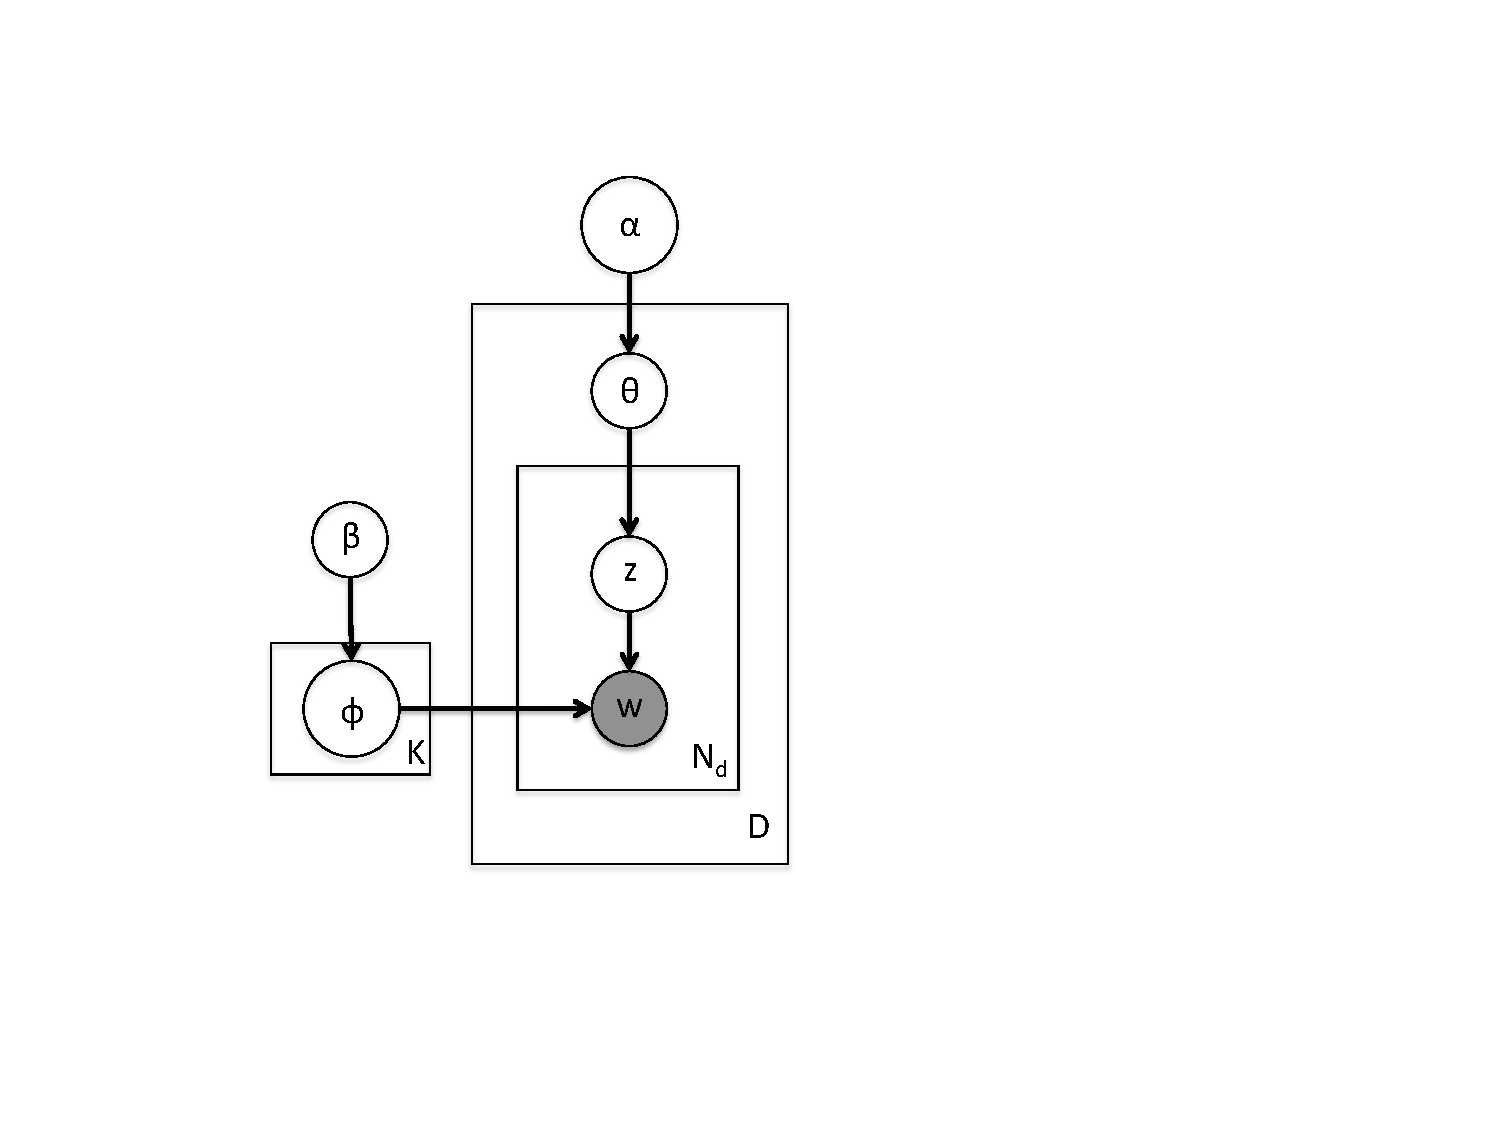
\includegraphics[trim = 40mm 35mm 80mm 25mm, clip, scale=0.4]{fig/lda_model.pdf} \label{fig:lda_model}}
        \subfigure{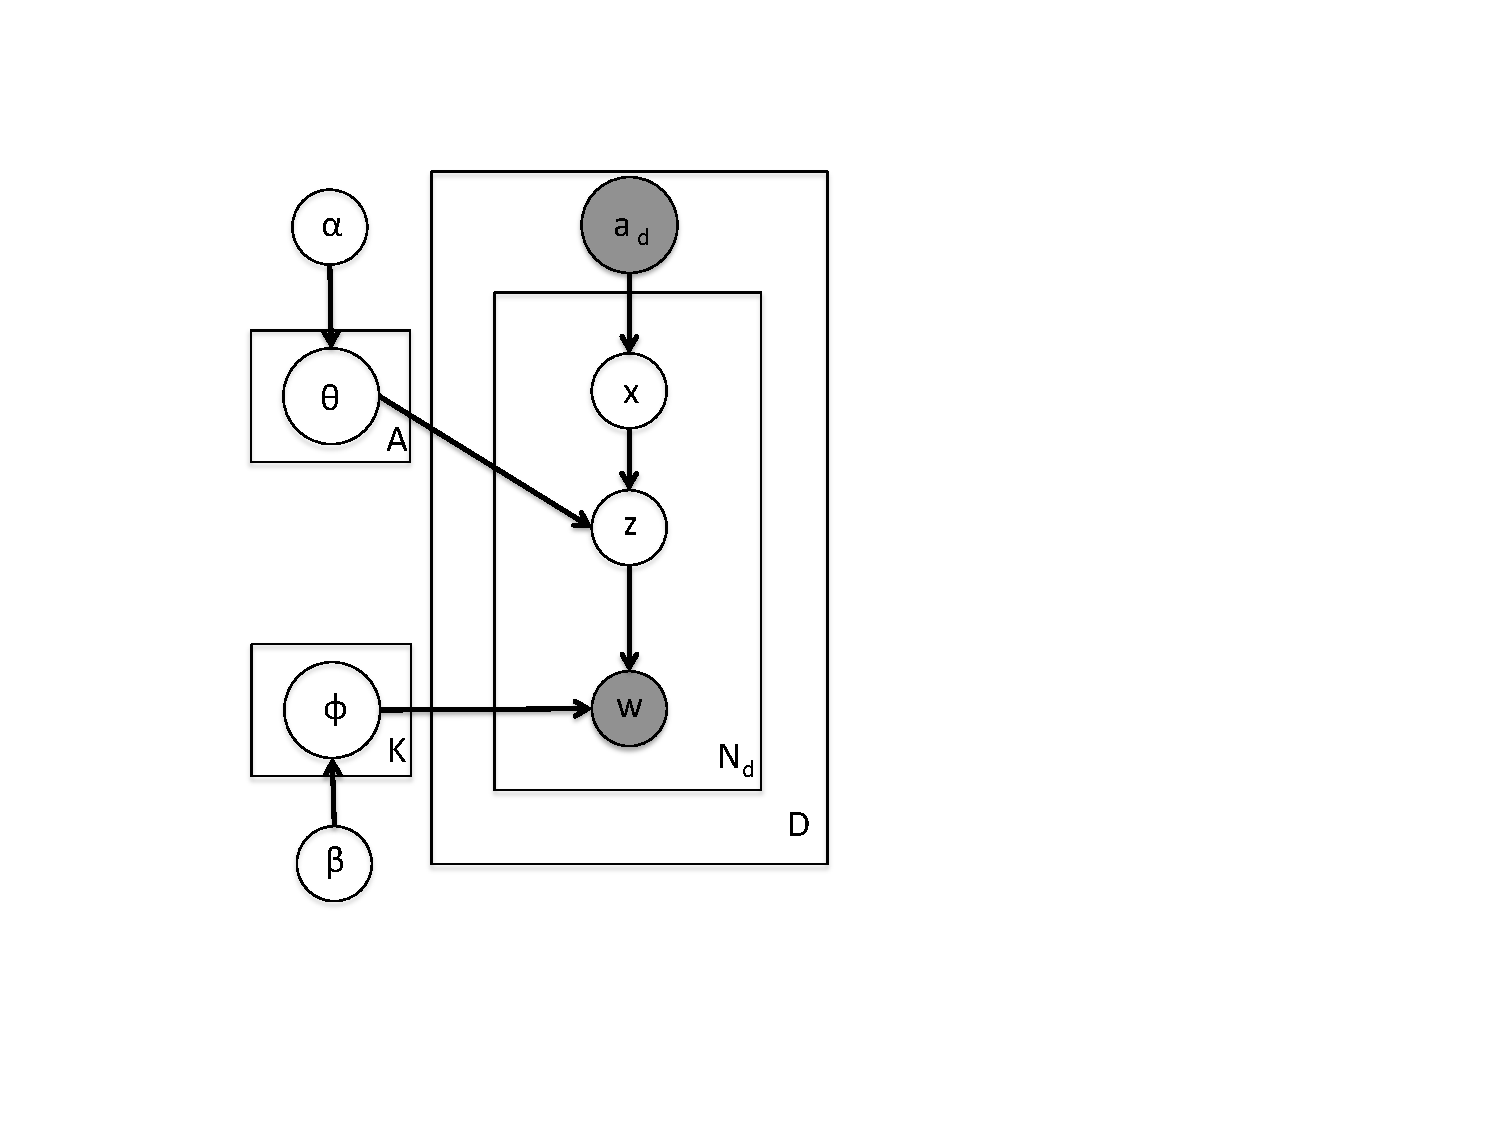
\includegraphics[trim = 40mm 35mm 70mm 25mm, clip, scale=0.4]{fig/at_model.pdf} \label{fig:at_model}}
        \subfigure{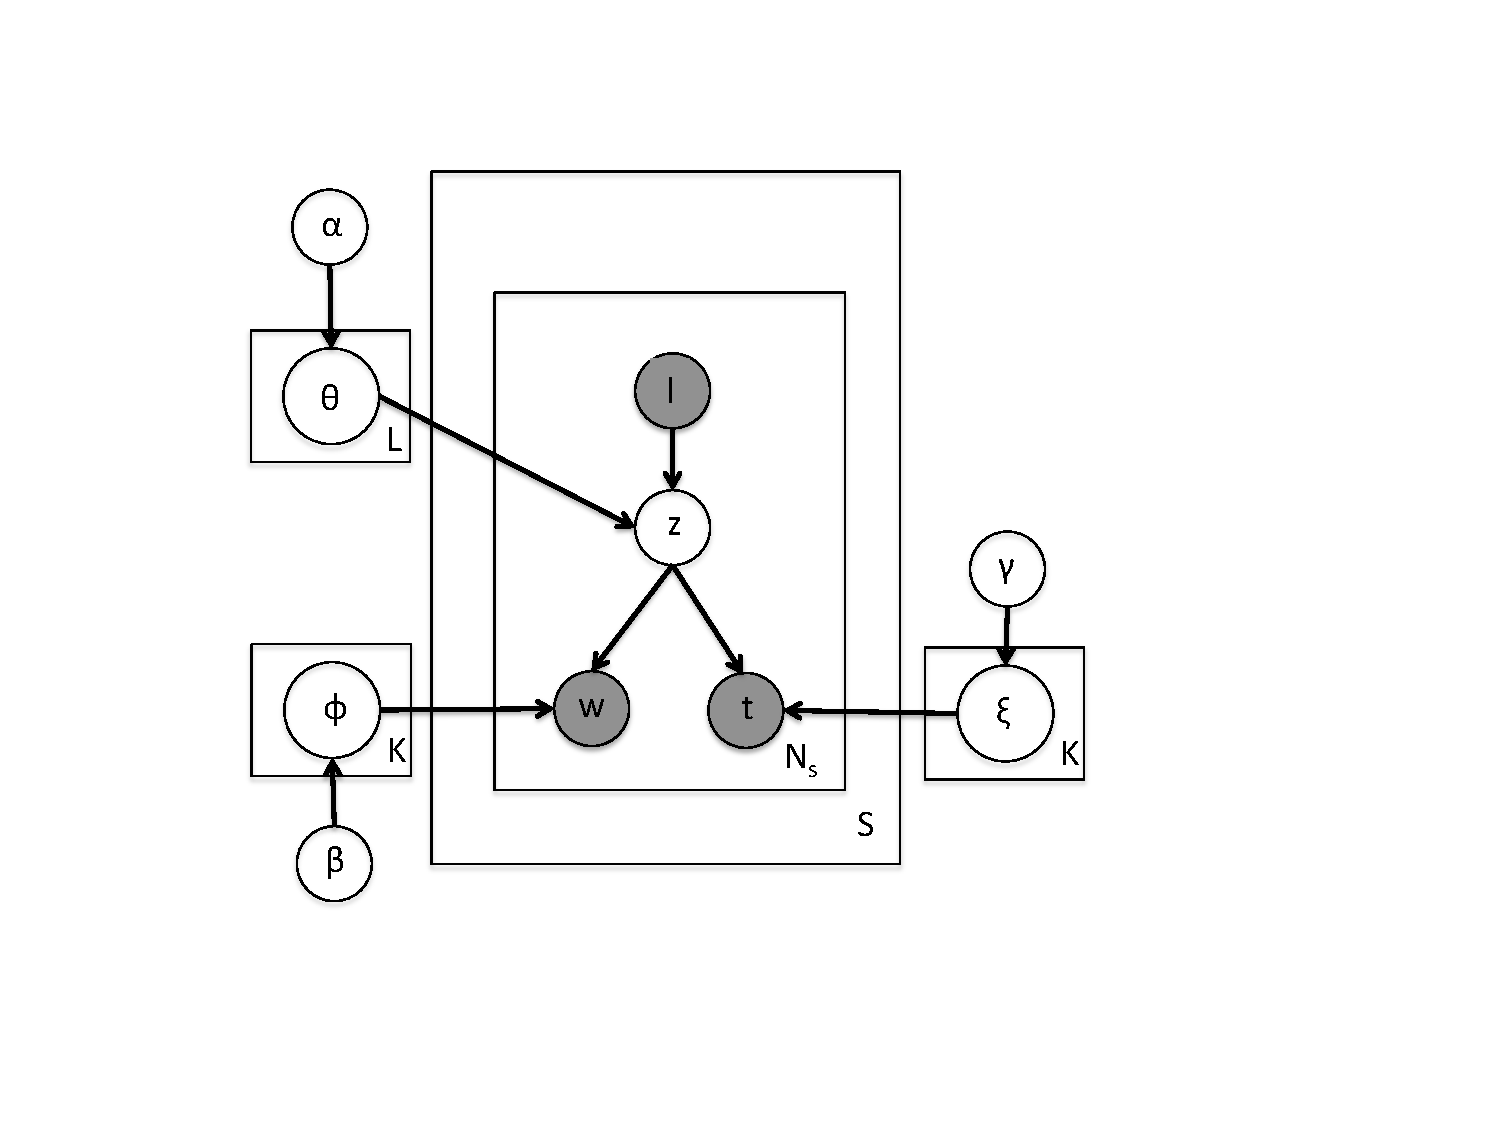
\includegraphics[trim = 30mm 35mm 70mm 25mm, clip, scale=0.4]{fig/stm_model.pdf} \label{fig:stm_model}}
\end{center}
\caption{Plate notation for three topic models: (a) Latent Dirichlet Allocation Model. (b) Author-Topic Model. (c) S-STAT Model.}
\label{fig:models}
\end{figure*}


\begin{table*}
\small \centering
\caption{Notation used in this paper.}
\begin{tabular}{c c}
\hline
{\bf Symbol} & {\bf Description}  \\
K & Number of topics  \\
S & Number of sources \\
V & Number of words \\
T & Number of discrete time-points \\
L & Number of locations \\
$N_s$ & Number of entries in each source $s$\\
$\psi_s$ & The multinomial distribution of locations specific to source $s$\\
$\theta_l$ & The multinomial distribution of topics specific to location $l$\\
$\phi_z$ & The multinomial distribution of words specific to topic $z$\\
$\xi_z$ & The multinomial distribution of time-points specific to topic $z$\\
$z_{si}$ & The topic associated with the $i$th entry from source $s$ \\
$l_{si}$ & The location associated with the $i$th entry from source $s$ \\
$w_{si}$ & The word associated with the $i$th entry from source $s$ \\
$t_{si}$ & The time-point associated with the $i$th entry from source $s$ \\
\hline
\end{tabular}
\label{tab:notation}
\end{table*}

\ \\{\bf \model generative proceess}
\begin{enumerate}
\item Draw $K$ multinomials $\phi_z$ from a Dirichlet prior $\beta$, one for each topic $z$;
\item Draw $K$ multinomials $\xi_z$ from a Dirichlet prior $\gamma$, one for each topic $z$;
\item Draw $L$ multinomials $\theta_l$ from a Dirichlet prior $\alpha$, one for each location $l$;
\item For each source  $s \in S$ and for each entry $i \in N_s$ with location $l_{si} \in L$:
\begin{enumerate}
\item Draw a topic $z_{si}$ from the multinomial $\theta_{l_{si}}$;
\item Draw a word $w_{si}$ from multinomial $\phi_{z_{si}}$;
\item Draw a time-point $t_{si}$ from multinomial $\xi_{z_{si}}$.
\end{enumerate}
\end{enumerate}

Each source entry is associated with a location $l_{si} \in L$ and we consider a distribution $\theta_{l_{si}}$ over topics that is randomly sampled from a Dirichlet with parameter $\alpha$. To generate each entry $i \in N_s$ for source $s$, first, a topic $z_{si}$ is chosen from the topic distribution $\theta_{l_{si}}$, and then, a word $w_{si}$ and time-point $t_{si}$ are generated by randomly sampling from the topic-specific multinomial distributions $\phi_{z_{si}}$ and $\xi_{z_{si}}$.  In our experiment we assume a fixed number of topics $K$.

As described in the above generative process, the posterior distribution of topics depends on the information from three modalities, i.e., the text, location and time. \model parametrization is:
\begin{align}
\theta_{l}|\alpha & \sim {\sf Dirichlet}(\alpha) \nonumber \\
\phi_{z}|\beta & \sim {\sf Dirichlet}(\beta) \nonumber \\ 
\xi_{z}|\gamma & \sim {\sf Dirichlet}(\gamma) \nonumber \\
z_{si}|l_{si},\theta_{l_{si}} & \sim {\sf Multinomial}(\theta_{l_{si}}) \nonumber \\
w_{si}|\phi_{z_{si}} & \sim {\sf Multinomial}(\phi_{z_{si}}) \nonumber \\
t_{si}|\xi_{z_{si}} & \sim {\sf Multinomial}(\xi_{z_{si}}) \nonumber
\end{align}

%The multinomial distribution over locations can be learned directly by the available data $N_s$ for each source. More precisely, given a source $s \in S$ we compute each parameter $p_{s,l}$ of the multinomial $\psi_s$  for each location $l \in L$ by taking its maximum likehood estimate, i.e., $p_{s,l} = {p}^{ML}_{s,l} = \frac{N_{l,s}}{N_{s}}$, where $N_{l,s}$ denotes the number of entries in $N_s$ associated with location $l$ and $N_s$ the total number of entries provided by source $s$.
As inference cannot be done exactly in \model, we employ a Gibbs sampling algorithm to perform approximate inference. Using a Dirichlet conjugate prior for the multinomial distributions allows us to easily integrate out $\theta$, $\phi$ and $\xi$.  In the Gibbs sampling procedure for estimating the parameters in \model, we need to calculate the conditional probability distribution $\Pr(z_{si}|{\bf w},{\bf t}, {\bf l}, {\bf z}_{-si}, \alpha, \beta, \gamma, {\bf \Psi})$ where ${\bf z}_{-si}$ represents the topic assignments for all entries in $s$ except the $i$-th entry. We begin with the joint probability of a data set and using the chain rule we obtain the conditional probability as:
\begin{align}
\label{eq:conditional}
&\Pr(z_{si}| \w,\tim,\loc,\z_{-si};\alpha,\beta,\gamma,\Psi) \nonumber \\
&= \frac{\Pr(z_{si}, w_{si}, t_{si}, l_{si}|\w_{-si},\tim_{-si},\loc_{-si},\z_{-si};\alpha,\beta,\gamma,\Psi)}{\Pr(w_{si}, t_{si}, l_{si}|\w_{-si},\tim_{-si},\loc_{-si},\z_{-si};\alpha,\beta,\gamma,\Psi)} \nonumber \\
& \propto \frac{n^{k,-(s,i)}_{w_{si}} + \beta_{w_{si}}}{\sum_{r = 1}^V n^{k,-(s,i)}_{r} + \beta_{r}} \cdot \frac{m^{k,-(s,i)}_{t_{si}} + \gamma_{t_{si}}}{\sum_{t = 1}^T m^{k,-(s,i)}_{t} + \gamma_{t}} \nonumber \\
& \cdot \frac{o^{k,-(s,i)}_{l_{si}} + \alpha_{l_{si}}}{\sum_{l = 1}^L o^{k,-(s,i)}_{l} + \alpha_{l}}
\end{align}
where $n^{z}_{r}$ denotes the number of times word $r$ was associated with topic $z$ across all sources and entries, $m^{z}_{t}$ denotes the number of times time-point $t$ was associated with topic $z$ across all sources, $o^z_l$ denotes the number of times location $l$ was associated with topic $z$ across all sources and their entries, and $-si$ in the superscript indicates that the current example has been excluded by the count summations. Notice, that since the location for the $(s,i)$-th entry is observed the distribution $\psi_s$ can be considered as a constant. A detailed derivation of Gibbs sampling for \model is provided in \Cref{sec:gibbs}. 

Once the sampler has converged, we can estimate the parameters of the multinomials $\theta$, $\phi$, and $\xi$ as follows:
\begin{align}
\label{eq:updates}
\theta_{l,z} = \frac{o^z_l + \alpha_l}{\sum_{z=1}^K o^z_l + \alpha_l} \nonumber \\
\phi_{z,v} = \frac{n^z_l + \alpha_l}{\sum_{v=1}^V n^z_v + \beta_v}  \\
\xi_{l,z} = \frac{m^z_t + \alpha_l}{\sum_{t=1}^T m^z_t + \gamma_t} \nonumber
\end{align}
The Gibbs sampling approximate inference for \model procedure is shown in Algorithm \ref{algo:gibbs}. For each entry in a set of event collection $\mathcal{X}$ we assign a hidden topic $z$ according to \Cref{eq:conditional}, and update the appropriate counts. After the sampling, we compute the distributions ${\boldsymbol \theta}$, ${\boldsymbol \xi}$ and ${\boldsymbol \phi}$ according to equation \Cref{eq:updates}. 

\begin{algorithm}[h]
\caption{\model Gibbs Sampling Approximate Inference}
\begin{algorithmic}[1]
\STATE {\bf Input:} $\mathcal{X}$: set of event entry collections; $N_{tier}$: number of iterations; 
\STATE {\bf Output:} ${\boldsymbol \theta}$: location-topic distributions; ${\boldsymbol \phi}$: topic-word distributions; ${\boldsymbol \xi}$: topic-timepoint distributions;
\STATE Initialize topic assignment randomly for all event entries in $\mathcal{X}$
\FORALL {$j$ to $N_{iter}$}
    \FORALL {$s \in S$}
    	\FORALL {$i \in N_s$}
		\STATE Draw $z_{si}$ from $\Pr(z_{si}| \w,\tim,\loc,\z_{-si};\alpha,\beta,\gamma,\Psi)$
		\STATE Update the counts $n^{z}_{r}$, $m^{z}_{t}$ and $o^z_l$
	\ENDFOR	
    \ENDFOR
\ENDFOR
\STATE Compute the posterior estimates ${\boldsymbol \theta}$, ${\boldsymbol \xi}$ and ${\boldsymbol \phi}$ as in \Cref{eq:updates}
\RETURN ${\boldsymbol \theta}$, ${\boldsymbol \xi}$, ${\boldsymbol \phi}$
\end{algorithmic}
\label{algo:gibbs}
\end{algorithm}


\section{Predicting Disease Outbreaks}
\label{sec:pred}
In this section, we describe how the posterior distributions learned by \model can be used to forecast outbreaks at a future time point $t$ for the set of locations present in $\mathcal{X}$. 
First, we show how to extract individualized predictions for each source-location pair in $\mathcal{P} = \bigcup_{s \in S}s \times L_s$ by detecting source content anomalies that indicate the emergence of a disease outbreak. Then, we present a randomized weighted majority voting algorithm for learning the accuracy of each source-based predictor for a certain location and fusing the individual source predictions.

\subsection{Source-based Outbreak Predictions}
\label{sec:source_pred}
Detecting an anomaly in the content of a source $s$ for a location $l$, requires reasoning about the relevance of the source's content to the discovered disease topics. We cast the latter problem as an instantiation of the {\em document classification}~\cite{strehl:2000} problem and show how the relevance between the content of a source and a topic can be instantiated using the {\em cosine similarity metric}.

For each topic $z \in K$, \model learns a distribution $\phi_z$ over all words in the vocabulary $V$. Moreover, following a similar approach to Matsubara et al.~\cite{matsubara:2012}, we extract the average occurrence rate $\bar{x}_w$ for each word $w \in V$ across all entries. Combining the above, one can construct an {\em average representative document} for each topic $z \in Z$, characterized by a vector $F_z$ that contains the expected occurrence frequency of each word $w \in V$ given the topic. In particular, we define the $w$-th entry of $F_z$ corresponding to word $w$ as $F_z,w = \bar{x}_w \cdot \phi_{z,w}$. Similarly, given the content source $s$ for a location $l$ at time $t$, one can derive a word frequency vector $F_{s,l,t}$ characterizing the content. Given the vectors $F_z$ and $F_{s,l,t}$ we define the relevance of the content of source $s$ for location $l$ at time $t$ to topic $z$ as:
\begin{equation}
{\sf Relevance}(s,z;l,t) = {\sf CosineSimilarity}(F_{s,l,t},F_z)
\end{equation}
where the cosine similarity of two vectors $A$ and $B$ is defined as:
\[
{\sf CosineSimilarity}(A,B) = \frac{A \cdot B}{\|A\| \|B\|}
\]

However, we want to predict disease outbreaks at future time points when the content of each source is not available to us. Therefore, given a source $s$, a location $l$ and a future time point $t$, we estimate the entries of $F_{s,l,t}$ by considering the expected frequency of each word. More precisely, let $\hat{F}_{s,l,t}[w]$ denote the expected frequency for word $w \in V$. To compute the expected frequency for $w$, we need to consider the probability of source $s$ publishing at a time $t$, denoted by $\Pr(t|s)$, the probability of source $s$ publishing for location $l$, denoted by $\Pr(l|s)$ and the probability that word $w$ was generated by any topic $z \in K$, given location $l$ and time point $t$. More precisely, we have that:
\begin{equation}
\hat{F}_{s,l,t}[w] = \Pr(t|s) \cdot \Pr(l|t)\cdot \sum_{z \in K}\phi_{z,w}\cdot \theta_{l,z} \cdot \xi_{z,t}
\end{equation}
where $\bar{x}_{w}$ denotes the average rate of occurrences of word $w$ in $\mathcal{X}$,  $\phi_{z,w}$, $\theta_{l,z}$, and $\xi_{z,t}$, can be retrieved by the output of \model,  and $\Pr(l|s)$ can be retrieved by the distribution $\psi_s$ learned from $\mathcal{X}$. Notice that $\xi_{z,t}$, i.e., the probability of topic $z$ being prominent at time $t$, and $\Pr(t|s)$ correspond to future time points and need to be estimated.  

According to the problem description in \Cref{sec:problem}, the available historical data spans up to time point $t-1$. Thus, we estimate the probability of the source publishing at a time $t$ by considering the weighted average publishing rate of the source:
\begin{equation}
\Pr(t|s) = \frac{\sum_{\tau = 1}^{t-1} \frac{1}{t - \tau}I(\tau,s)}{\sum_{\tau = 1}^{t-1} \frac{1}{t - \tau}}
\end{equation}
where $I(s,\tau)$ is an indicator variable equal to one if the source $s$ published at time $\tau$ and zero otherwise. To estimate the probability $\xi_{z,t} \mbox{with } z \in \{1, 2, \dots, K\}$, we use the values of distribution $\xi_{z}, \forall z \in K$ corresponding to past time points. In particular, we use an autoregressive model over the values of topic $z$ for the $n$ previous time intervals, denoted by $\xi_{z,t-1},\xi_{z,t-2},\dots,\xi_{z,t-N}$.We have:
\begin{equation}
\xi_{z,t}=a_1 \cdot \xi_{z,t-1}+a_2\cdot \xi_{z,t-2}+\dots +a_n\cdot \xi_{z,t-n}
\end{equation}
where $a_1,a_2,.....,a_n$ are the regression coefficients.


%Similarly, given the set of words present in the articles provided by source $s$ for a location $l$ at time $t$, one can derive a source-location based distribution $P({\bf w};s,l,t)$ over all words in $V$ as described below.  Given $\phi_z$ and $P({\bf w};s,l,t)$ we define the relevance of a topic $z$ to source $s$ for location $l$ as the normalized distance between the distributions $\phi_z$ and $P({\bf w};s,l,t)$. Next, we discuss how the probability distribution $P({\bf w};s,l,t)$ can be estimated for future time points and we formally present a distance metric based on KL-divergence for defining relevance.
%
%Given a source $s \in S$, a location $l \in L$ and a time point $t$ each parameters $p_{w,s,l,t}, \forall w \in V$ of the distribution $P({\bf w};s,l,t)$, can be estimated as $p_{w,s,l,t} = \frac{x_{w,s,l,t}}{\sum_{w \in V} x_{w,s,l,t}}$, i.e., the fraction of the number of articles $x_{w,s,l,t}$ by $s$ at time $t$ that correspond to location $l$ and mention the word $w$ over the total number of articles in $s$ at time $t$ for location $l$. Intuitively, when given a topic $z$ and a future time point $t$, the appearance count of a word in source $s$ for location $l$ at time $t$ is equal to the average occurrence rate of the word, regardless of the source, multiplied by the probability of that word being generated by topic $z$ multiplied by the probability that this topic is relevant to location $l$ and the probability of that topic being prominent at time $t$, multiplied by the probability of location $l$ appearing in $s$. Thus to compute the overall estimated appearance count of a word $w$ we need to sum over all topics. We have:
%
%\begin{equation}
%x_{w,s,l,t} = \bar{x}_{w}\cdot \sum_{z = 1}^K \phi_{z,w}\cdot \theta_{l,z} \cdot \xi_{z,t} \cdot \Pr(l|s) 
%\label{eq:est_word}
%\end{equation}
%where $\bar{x}_{w}$ denotes the average rate of occurrences of word $w$ in $\mathcal{�}{X}$, and $\phi_{z,w}$, $\theta_{l,z}$, and $\Pr(l|s)$ can be retrieved by the distribution $\psi_s$ used in  \model. 
%
%However, $\xi_{z,t}$, i.e., the probability of topic $z$ being prominent at time $t$, corresponds to a future time point and needs to be estimated. We use the values of distribution $\xi_{z}, \forall z \in K$ corresponding to past time points to forecast the values $\xi_{z,t} \mbox{with } z \in \{1, 2, \dots, K\}$. We use an autoregressive model over the values of topic $z$ for the $n$ previous time intervals, denoted by $\xi_{z,t-1},\xi_{z,t-2},\dots,\xi_{z,t-N}$.We have:
%\begin{equation}
%\xi_{z,t}=a_1 \cdot \xi_{z,t-1}+a_2\cdot \xi_{z,t-2}+\dots +a_n\cdot \xi_{z,t-n}
%\end{equation}
%where $a_1,a_2,.....,a_n$ are the regression coefficients.
%
%To determine how relevant a topic is to the content of source $s$ for location $l$, we cast the problem as a document categorization topic and consider the normalized distance between distributions $\phi_z$ and $P({\bf w};s,l,t)$ to be equal to their symmetric KL distance~\cite{bigi:2003}.  More precisely, given a topic $z$ and the content of a source $s$ for location $l$ at time $t$, denoted by $s_{l,t}$ we have that the topic to source relevance is:
%
%\begin{equation}
%{\sf Relevance}(z, s_{l,t}) = 1 - \frac{KLD(\phi_z,s_{l,t})}{KLD(\phi_z,\emptyset)}
%\end{equation}
%where $KLD(\phi_z,s_{l,t})$ denotes the KL distance between distributions $\phi_z$ and $P({\bf w};s,l,t)$, and $KLD(\phi_z,\emptyset)$ denotes the KL distance between the distribution for topic $\phi_z$ and the empty document. For the empty document we define its word distribution as $P(w; \emptyset) = \epsilon, \forall w \in V$ where $\epsilon$ corresponds to a small positive constant. The symmetric KL distance between $\phi_z$ and $P({\bf w};s,l,t)$ is defined as:
%
%\begin{equation}
%KLD(\phi_z, s_{l,t}) = \sum_{w \in V} (P(w;z) - P(w;s,l,t))\cdot \log\frac{P(w;z)}{P(w;s,l,t)} \nonumber
%\end{equation}
%Due to space limitations we refer the reader to Bigi~\cite{bigi:2003} for details. 

Finally, to detect if the source-topic relevance for a future time point constitutes an anomalous points we use one-class SVMs~\cite{schoelkopf:99} (OCSVM). A OCSVM maps input data $X$ into a high dimensional feature space $H$ via a kernel $\Phi: X \rightarrow H$ and finds the maximal margin hyperplane which best separates the training data from the origin. The classification rule corresponds to $f(x) = {\sf sign}(\mathbf{w}\Phi(x) - b)$, where $\mathbf{w}$ is a weight vector and $b$ is a bias term. We use this classification rule to detect if a new point $x$ is an anomalous point (i.e., $f(x) < 0$) or not. 

We train a separate OCSVM for each source, location and disease topic triplet and forecast outbreaks on a weekly basis. The features used in each OCSVM correspond to the predicted relevance of the source's content to each topic for the past time points. To improve the robustness of each OCSVM, we exclude the time points that correspond to actual disease outbreaks from our training data. For this, we make use of a gold standard report (GSR) which gives ground truth determinations of whether a disease incidence (Hantavirus) happened in a given location at a time point included in $T$. The GSR is determined by analysts poring over multiple news sources and studying bulletins issued by health reporting organizations such as ProMED~\cite{probmed}.  This approach thus predicts  {\em if} a disease outbreak will happen based on the data provided by a source and {\em where} it will happen (since we are training and forecasting for each location). For the {\em when} since we are predicting for an epi week we adopt a standard relative date within the epi week to be the date at which the rare disease incidence will occur, and tune it using cross-validation. 



\subsection{Fusing Multiple Predictions}
\label{sec:integration}

Until now, we discussed how the events provided by each source can be used to derive an outbreak prediction when considering each individual source as an expert. However, our final goal is to detect the incidence of a particular disease for a specific location. Thus, we fuse the predictions of all sources into a single prediction for each location $l \in L$ at time $t$ using a randomized weighted majority voting algorithm\cite{arora:2012}.

Given time $t$ in the future, we focus on a location $l$ and view each source $s \in S$ as an expert providing a prediction $d_s \in [-1,1]$ with the value $-1$ corresponding to the emergence of an outbreak. We also assign a weight $w_s$ to each source. Given the predictions of all sources, we predict yes/no for an outbreak at location $l$ by taking the majority vote $\sum_{s \in S} w_s \cdot d_s$.  We learn the weight $w_s$ for each source using the randomized multiplicative weights update algorithm shown in Algorithm \ref{algo:mw}.

\begin{algorithm}[h]
\caption{Multiplicative Weights Update for Source Accuracy}
\begin{algorithmic}[1]
\STATE {\bf Input:} $N_l$: set of sources for location $l$; ${\bf D_l}$: training points;
\STATE {\bf Output:} $\bf{W}$: weights for sources in $N_l$
\STATE $T \leftarrow \lceil \frac{4\ln(|N_l|)}{\epsilon^2} \rceil$ {\em /* Initialize number of epochs */}
\STATE Initialize all weights $W$ to 1
\FORALL {$t$ to $\{1, 2, \dots, T\}$}
    \FORALL {$d \in {\bf D_l}$}
    	\FORALL {$i \in N_s$}
		\STATE {\em /* Construct the expert distribution $\mathcal{D}$*/}
		\STATE $\mathcal{D} = \{p_1,p_2, \dots, p_{|N_l|}\}, ~p_i = \frac{W_i}{\sum_{j \in N_l} W_j}, \forall i \in N_l$
		\STATE Draw an expert $k$ from $\mathcal{D}$
		\STATE Use expert $k$ to get a prediction $d_k$ for point $d$
		\IF {the expert makes a mistake}
			\STATE $W_k \leftarrow W_k\cdot (1 - \epsilon)$ {\em /* Decrease the weight */}
		\ENDIF
	\ENDFOR	
    \ENDFOR
\ENDFOR
\RETURN ${\bf W}$
\end{algorithmic}
\label{algo:mw}
\end{algorithm}

We consider a location $l$ and a disease topic $z$, and construct the necessary input for the multiplicative weights update algorithm. More precisely, we identify the set of sources that can be considered as experts for location $l$, i.e., sources for which $\Pr(l|s) \geq 0$, and then we construct the set of training points  ${\bf D}$ by considering the reported outbreaks in GSR that correspond to location $l$ and topic $z$. More precisely, we populate ${\bf D_l}$ with tuples of the form $(time point, outbreak)$ for all historical time points present in $\mathcal{X}$, while setting the value of $outbreak$ to $-1$ if an actual outbreak was reported and $1$ otherwise.

Given the input described above, the algorithm proceeds in an iterative fashion updating the weights of the sources based on the accuracy of their predictions. In particular, the algorithm iterates over all training points in ${\bf D}$ for $T$ epochs (Ln. 6 - 7). The number of epochs depends on the number of experts and is initialized to $\lceil \frac{4\ln(|N_l|)}{\epsilon^2} \rceil$ (Ln. 3) in order to achieve the standard error guarantees of the multiplicative weights update algorithm~\cite{arora:2012}. At each iteration, the algorithm constructs a probability distribution over the experts by normalizing their corresponding weights (Ln. 9) and samples a single expert from that distribution (Ln. 10) to form the final prediction for the corresponding training point. If the expert is mistaken, it's corresponding weight is reduced in a multiplicative fashion (Ln. 13). Finally, the algorithm outputs the weights corresponding to the accuracy of each source, which are later used to fuse the individual source predictions for future time points. The process is repeated as more ground-truth data are becoming available through GSR.




\section{Experimental Evaluation}
\label{sec:exp}
We present an empirical evaluation of the proposed framework: The main questions we seek to address are: (1) how effective is the proposed topic model in identifying disease topics, and in discovering the corresponding spatio-temporal patterns, (2) how accurately can the proposed techniques forecast disease outbreaks, and (3) whether leveraging the varying authoritativeness levels of data sources for different locations can improve the accuracy of outbreak predictions. We empirically study these questions using real-world data focusing on rare-disease incidences in countries in Latin America.

%In this section we present an empirical evaluation of our proposed models 
%- location-based model and source-based model in detecting hantavirus outbreaks.
%The main questions we seek to address are:
%
%\begin{enumerate}
%  \item How can we interpret and identify different disease topics discovered
%    by the topic model
%  \item How early and accurately can our proposed models forecast Hantavirus 
%    outbreaks
%  \item How can we evaluate the relative importance of sources and/or experts 
%    in detecting hantavirus outbreaks, for a particular location and 
%    at a specific time.
%\end{enumerate}
\subsection{Experimental Setup}
\noindent{\bf Data:} We consider a dataset corresponding to a corpus of public health-related news articles and tweets extracted from HealthMap~\cite{healthmap}, a prominent online source of news articles and tweets for disease outbreak monitoring and real-time surveillance of emerging public health threats. In this paper, we focus on HealthMap articles from Latin America


. HealthMap~\cite{healthmap}  The dataset we have used for training our models is the HealthMap [?] (www.healthmap.org) 
corpus. HealthMap is a prominent online source of news articles and tweets for 
disease outbreak monitoring and real-time surveillance of emerging public health
threats. In operation since September 2006, HealthMap system captures outbreak 
as well as disease-related warning data from over 50,000 electronic media sources.
Thus HealthMap dataset has the potential to be used as an early detection system for disease outbreaks,
even from areas which is relatively inaccessible to traditional global public health efforts.
HealthMap system also supports multiple languages, currently it monitors disease outbreak information
sources in Spanish, English, Arabic, Portuguese, Russian, Chinese and French. Using this service 
we receive various disease-related news documents as a daily feed.

{\bf Input Setup and Preprocessing:}

Our corpus of public health-related news articles is drawn from HealthMap dataset
introduced in the above section. In our experiments we are focusing on the HealthMap articles of 
Latin America.  For Latin America, HealthMap articles provide monitoring and real-time surveillance 
information about multiple diseases like Swine Flu H1N1, Dengue, Avian Influenza, Hantavirus, Chagas and many more.

Content of each HealthMap article is enriched and extracted tokens and/or words are fed thorugh a number of preprocessing steps 
like stopword removal to remove as much unwanted words as possible. HealthMap also 
tags each article with a (lat, long) information, URL information and a date. From the (lat, long) information, 
we infer the state and country of the article and the URL information
helps in determing the source and/or publisher of the article. Thus for each article we can extract the following information:
word count, location, source and timestamp. 

{\bf *Talk to theo and take some suggestions about writing this
paragraph*}




{\bf Models:} We evaluate the following models:

\begin{itemize}

\item Source-based Model (S-STAT): This model corresponds to the source-based 
  disease outbreak detection approach. This model has the following sub-models:
  1) Tensor-based Topic Model which gives different topic distributions 
  as output, 2) then the Prediction Model which calculates the topic cosine similarity 
  values corresponding to each source and location for the future timepoint and 3) finally the multiplicative 
  weights algorithm makes the final prediction for a particular location by calculating 
  the weighted sum of the OCSVM prediction of the relevant sources for that location.
  The weights are assigned to each expert and/or source based on its accuracy of prediction 
  over the historical timepoints.
\item Location-based Model (L-STAT): There is no concept of source and/or expert 
  in this model. It has the following sub-models: 1) The Topic Model, and 2) then 
  the Prediction Model which computes the topic cosine similarity values for each location for the future timepoint
  and 3) the OCSVM Model which predicts whether the predicted cosine similarity value is an anomalous point or a normal
  point with respect to the historical similarity values. If it is an anomalous point, the model generates a warning.
\item Base Rate Model (BRM): We also compare the performance of our framework against a base rate model (BRM). This
    model assumes a fixed rate for the occurence of hantavirus outbreaks for each country and each 
    month. To determine this rate, the model extracts the average frequency of outbreak occurrences
    reported over a past time window of four months. BRM reports disease outbreaks for that country at 
    a frequency equal to the extracted rate. Alerting dates are assigned to the beginning of each month
    while events dates are assigned uniformly at random to a day within the corresponding month. (Thus
    lead time is not a meaningful criterion to evaluate the BRM.) The performance of BRM is enhanced
    by taking the average performance over 25 independent runs.
\end{itemize}

All models are implemented in Python and the evaluation is performed on an Intel(R) Xeon(R) CPU E7- 4870 @2.40GHz/64bit/1TB machine.


\subsection{GSR}

The Ground Truth Data for disease incidences we used for evaluating our models is the Gold Standard Report (GSR). 
GSR is organized by an independent third party (MITRE), not the authors of this 
paper. Using Human Analysts, MITRE surveys multiple Latin American and/or International 
News Sources and study bulletins issued by health-reporting organizations such 
as PROMED [?] or CDC [?] to determine confirmed Hantavirus outbreaks. For each 
Hantavirus outbreak, MITRE provides the following information: 
\begin{enumerate}
  \item location information of the outbreak (Country, State and City)
  \item Event date (date at which the disease incidence has occured or outbreak has started)
  \item the earliest reported date in the news
  \item the news source reporting the disease incidence
  \item a small description of the disease incidence
\end{enumerate}

The analyst starts by reading headlines of an article and if a significant disease incidence is discovered
or inferred the analysts will skim through the remainder of the article to determine if a notable event is 
described therein. If such an event is discovered, the analyst will extract and 
encode relevant information given above about that event into a GSR template. In determining disease
incidences, the analysts also adopt a 6-month rule. More specifically, if a news report is 
for the same disease, in the same city within six months of the last report, then it 
is not a new event and will not appear in the GSR; otherwise it is a new event and will be captured in the GSR.
Figure 2 shows the distribution of confirmed Hantavirus incidences in four countries of Latin America (Chile, Argentina, Brazil and Uruguay)
from January 2013 to March 2014.

\begin{figure}[h!]
      \centering
          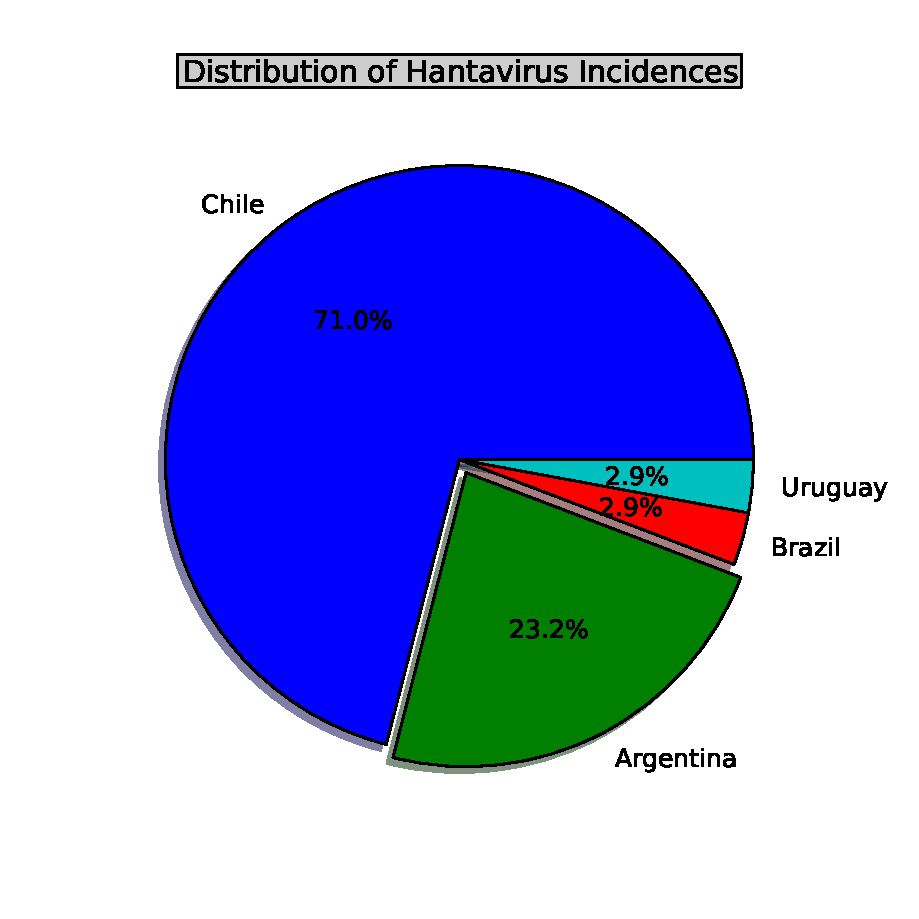
\includegraphics[width=0.5\textwidth]{fig/hanta_dist.pdf}
    \caption{Hantavirus Outbreak Distribution in four countries of Latin
  America (Chile, Argentina, Brazil, Uruguay) from January 2013 to March
  2014}
    \end{figure}

\subsection{Evaluation Metrics}

We adopt three key measures of performance (Quality Score, F1 score and Lead Time). Evaluation for a model is done 
on a monthly basis. More Specifically, the warnings and/or alerts generated from a model in a particular month
are evaluated against the GSR events in that month. Given our alerts, we compute the Recall and Precision at a country level, 
grouping together alerts for locations in the same country. Using the Recall 
and Precision values, we calculate the F1 score as $F_{1} = (2 * Precision * Recall) / (Precision + Recall)$.  

We also compute an average warning quality for each country. Each prediction for a location in 
the country under consideration is assigned a Quality Score $Q = (4/3) * (1 + a_{loc} + a_{date})$, where $a_{loc}$
and $a_{date}$ denote the location and date accuracy of the prediction. For calculating $a_{loc}$ we use a three-level
topology. At the top level is the country, the second level is the province, state, region, or department, or the 
next largest administrative division, and the third level is the city. The models will generate their 
warning using this typology, i.e. the warning will be in the form of a triple, (country, province or state, city). 
For rare disease, we do not have enough resolution at the city level, so the models predict upto the state level and
keeps the city name "-" in the warning. The evaluation script compares the warning location with 
the GSR location, to get $(x_{1}, x_{2}, x_{3})$, where $x_{1}$ is the country comparison, $x_{2}$ is the province 
or state comparison (if the GSR has that level of specificity), and $x_{3}$ is the city comparison 
(if the GSR has that level of specificity). $x_{i} = 0$ if they do not match, $x_{i} = 1$ if they do. If 
either one of the GSR entry or the warning entry is blank and the other is not, xi = 0. If 
both are blank, xi = 1. The match between the warning location and the GSR 
location is:  

    $a_{loc} = 1/3 x_{1} + 1/3 x_{1} x_{2} + 1/3 x_{1} x_{2} x_{3}$

Note that if $x_{1} = 0$ (i.e. the warning misses the country level location), then $a_{loc} = 0$. If 
all the entries match, then $a_{loc} = 1$. Note also that a warning is penalized if it is underspecified or overspecified.
The $a_{date}$ is calculated as $a_{date} = 1-min(|predicted date -
actual event date|, 7)/7$.
The Quality Score takes values between 0 and 4. 

Finally, we consider the lead time of our predictions, which is calculated as the
time between the alerting date in the warning and the actual date of reporting of the outbreak (not the incidence
date of the outbreak).

\paragraph{\bf Mapping Warnings to Events} Since there could be multiple
events (and/or alerts) in a given month, a strategy is necessary to map events to alerts. We
conduct a maximum bipartite matching between events and alerts where i) an edge
exists if the alert was issued prior to the reporting date of the event, ii) the
weight on the edge denotes the putative quality score. 


\subsection{Model Paramater Settings}

For the Topic Model we set Dirichlet parameter 
$\alpha = 2/K$ (prior on topic given location) where K is the number of topics, 
Dirichlet parameter $\beta = 0.01$ (prior on word given topic) and Dirichlet 
parameter $\gamma = 0.01$ (prior on time given topic). These Dirichlet Hyperparameter 
settings are typical for those used for analyzing hidden topics in datasets 
and will be almost similar to values that one can learn by sampling or optimization. 
For selecting the number of topics (K), we evaluated the Topic Model with 8, 12 and 15 topics. 
We find that setting $K=12$ results in more meaningful clustering of the hidden topics.  


For one-class SVM we use a parameter search algorithm to find the exact kernel and its associated 
set of parameters for each location and source in case of source-based model 
and for each location in case of location-based model. We first construct the 
training set based on non-disease points to be fed to the one-class SVM.
For each kernel ("polynomial" and "rbf") we start with a valid range of associated paramters
and for each combination of the parameters for each kernel, we calculate two types of error:
\begin{enumerate}

  \item \textbf{Normal Error} : This error is the sum of the error in predicting 
    the  normal and/or non-disease points calculated via the LOOCV method.
  \item \textbf{Anomalous Error} : This error is the sum of the error in predicting the anomalous and/or disease points
\end{enumerate}

For certain locations we may have no anomalous and/or disease points, i.e. there 
has been no hantavirus incidences in that location in the near past. For these 
locations we only consider the normal error. For locations where we have both normal 
and anomalous historical points, we evaluate the weighted sum of both the errors. We select 
the parameter combination which gives us the minimum overall error.

For the multiplicative weights algorithm the past window size over which we 
calculate the accuracy of each relevant source and/or expert for a location is set
to be 5 months. 

\subsection{Disease Topic Discovery}

The output of the Topic Model provides us the following information: location 
distribution over topics, topic distribution over words and Topic Distribution 
over time. Now the question is: How can we interpret and/or identify these hidden 
disease topics or what is the disease focus of each hidden topic? We accumulate a fixed 
vocabulary of health-related keywords such as "gripe" (flu), "h1n1", "dengue", "aegypti", "mosquitos",
"hanta", "hantavirus", "roedores" (rodents) and many more. For each hidden topic, 
we analyze the topic-word probability of these keywords to identify the disease
focus of the topic. More Specifically, under each topic we rank the keywords 
based on its probability values and we can infer the topic interpretation by 
looking at the top-ranked keywords under that topic. 

\begin{figure*}[ht]
\begin{center}
        \subfigure{
\includegraphics[scale=0.27]{figures/topic_12_cloud.pdf}\label{fig:topic_12_cloud}}
        \subfigure{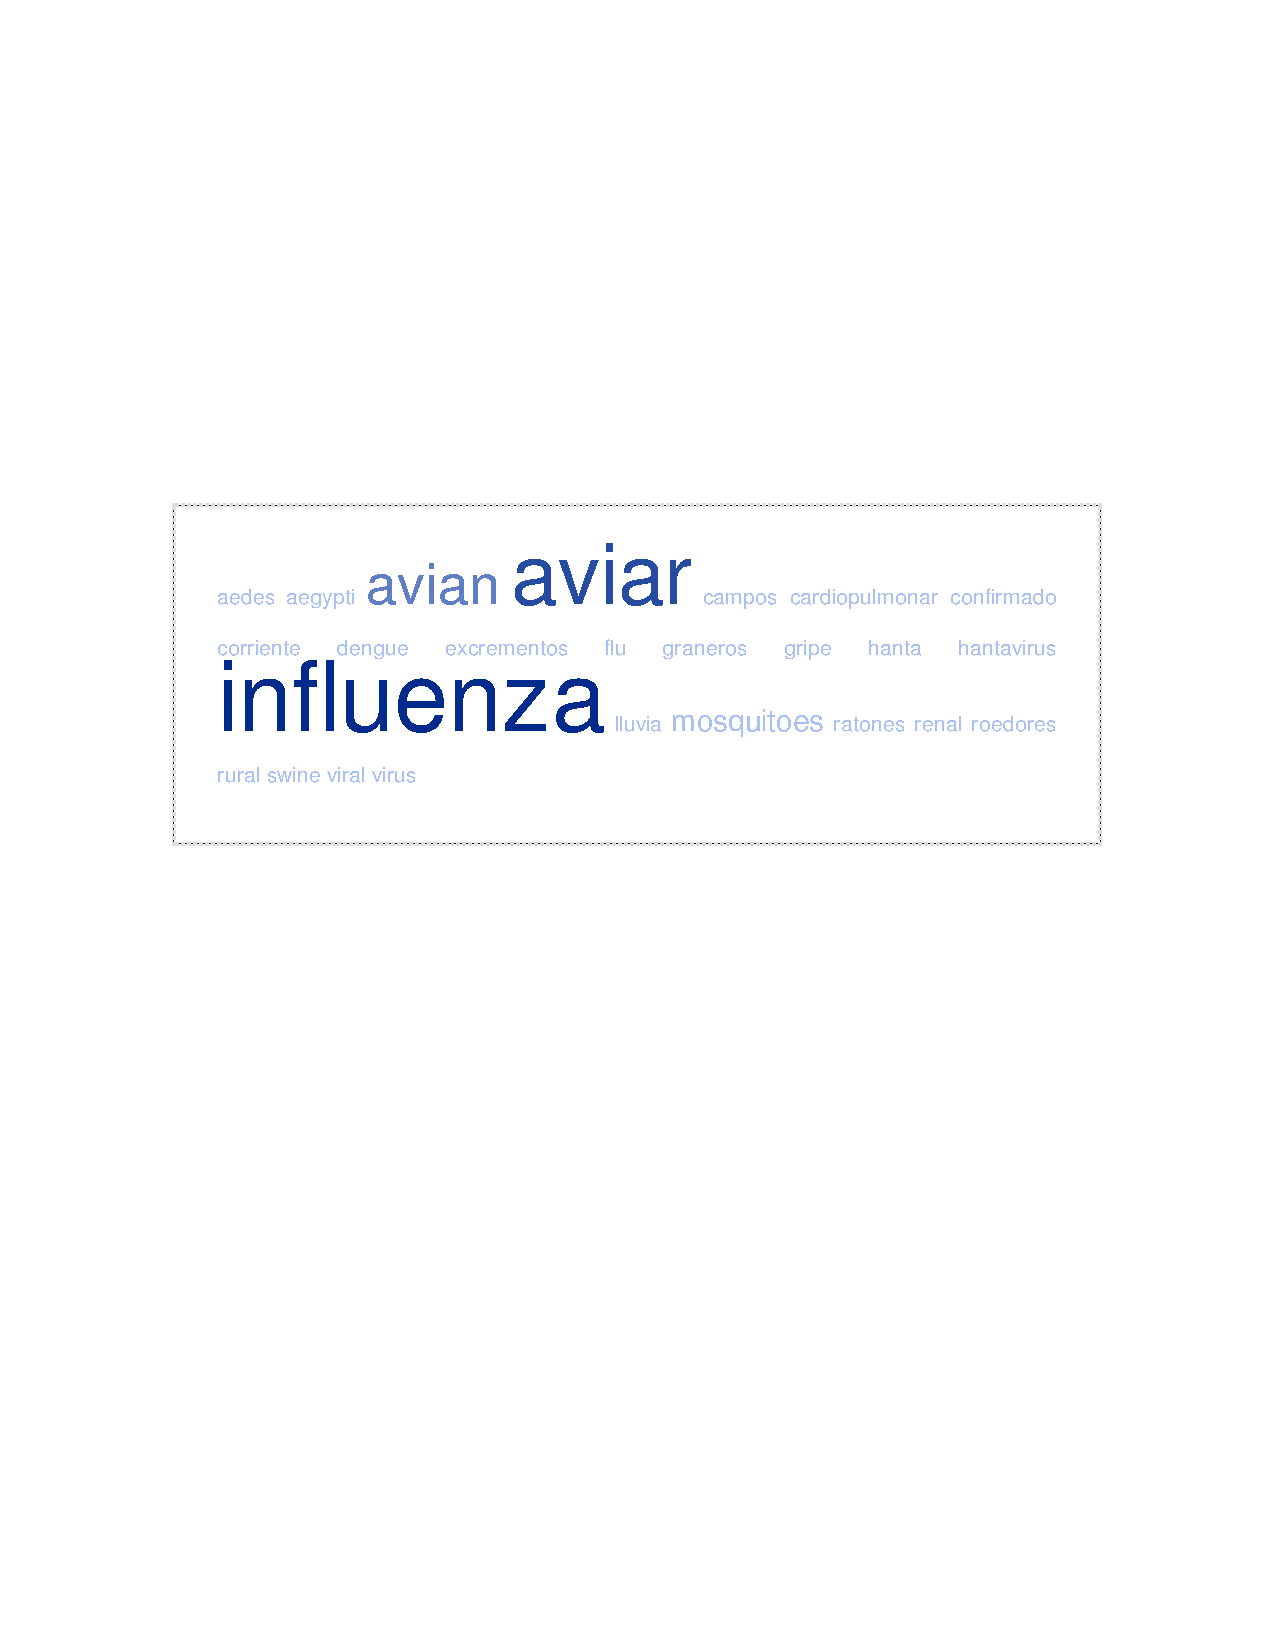
\includegraphics[scale=0.27]{figures/topic_9_cloud.pdf} \label{fig:topic_9_cloud}}
        \subfigure{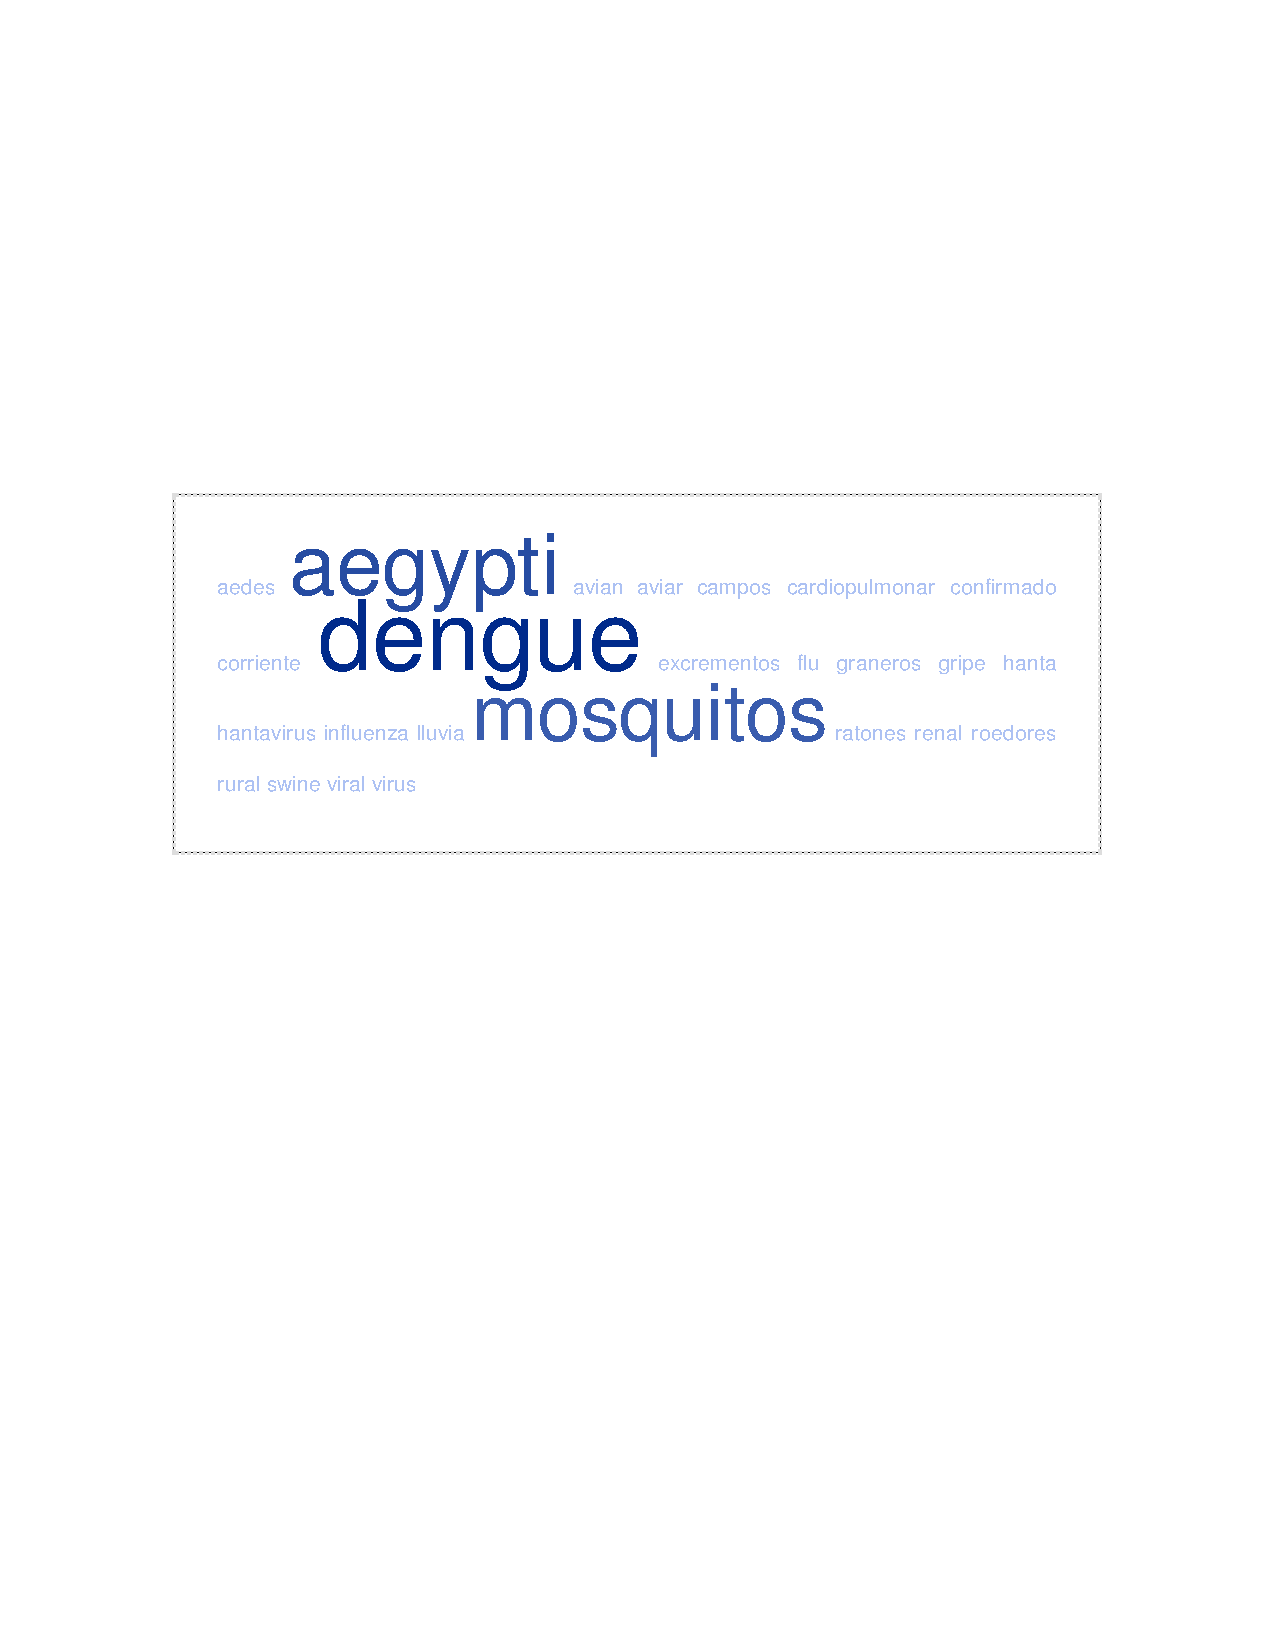
\includegraphics[scale=0.27]{figures/topic_10_cloud.pdf}\label{fig:topic_10_cloud}}
\end{center}
\caption{Word Clouds of Common Disease Topics (a) Topic 12 (Swine Flu) (b) Topic 9 (Avian Flu) (c) Topic 10 (Dengue)}
\label{fig:Common_clouds}
\end{figure*}

\begin{figure*}[ht]
\begin{center}
        \subfigure{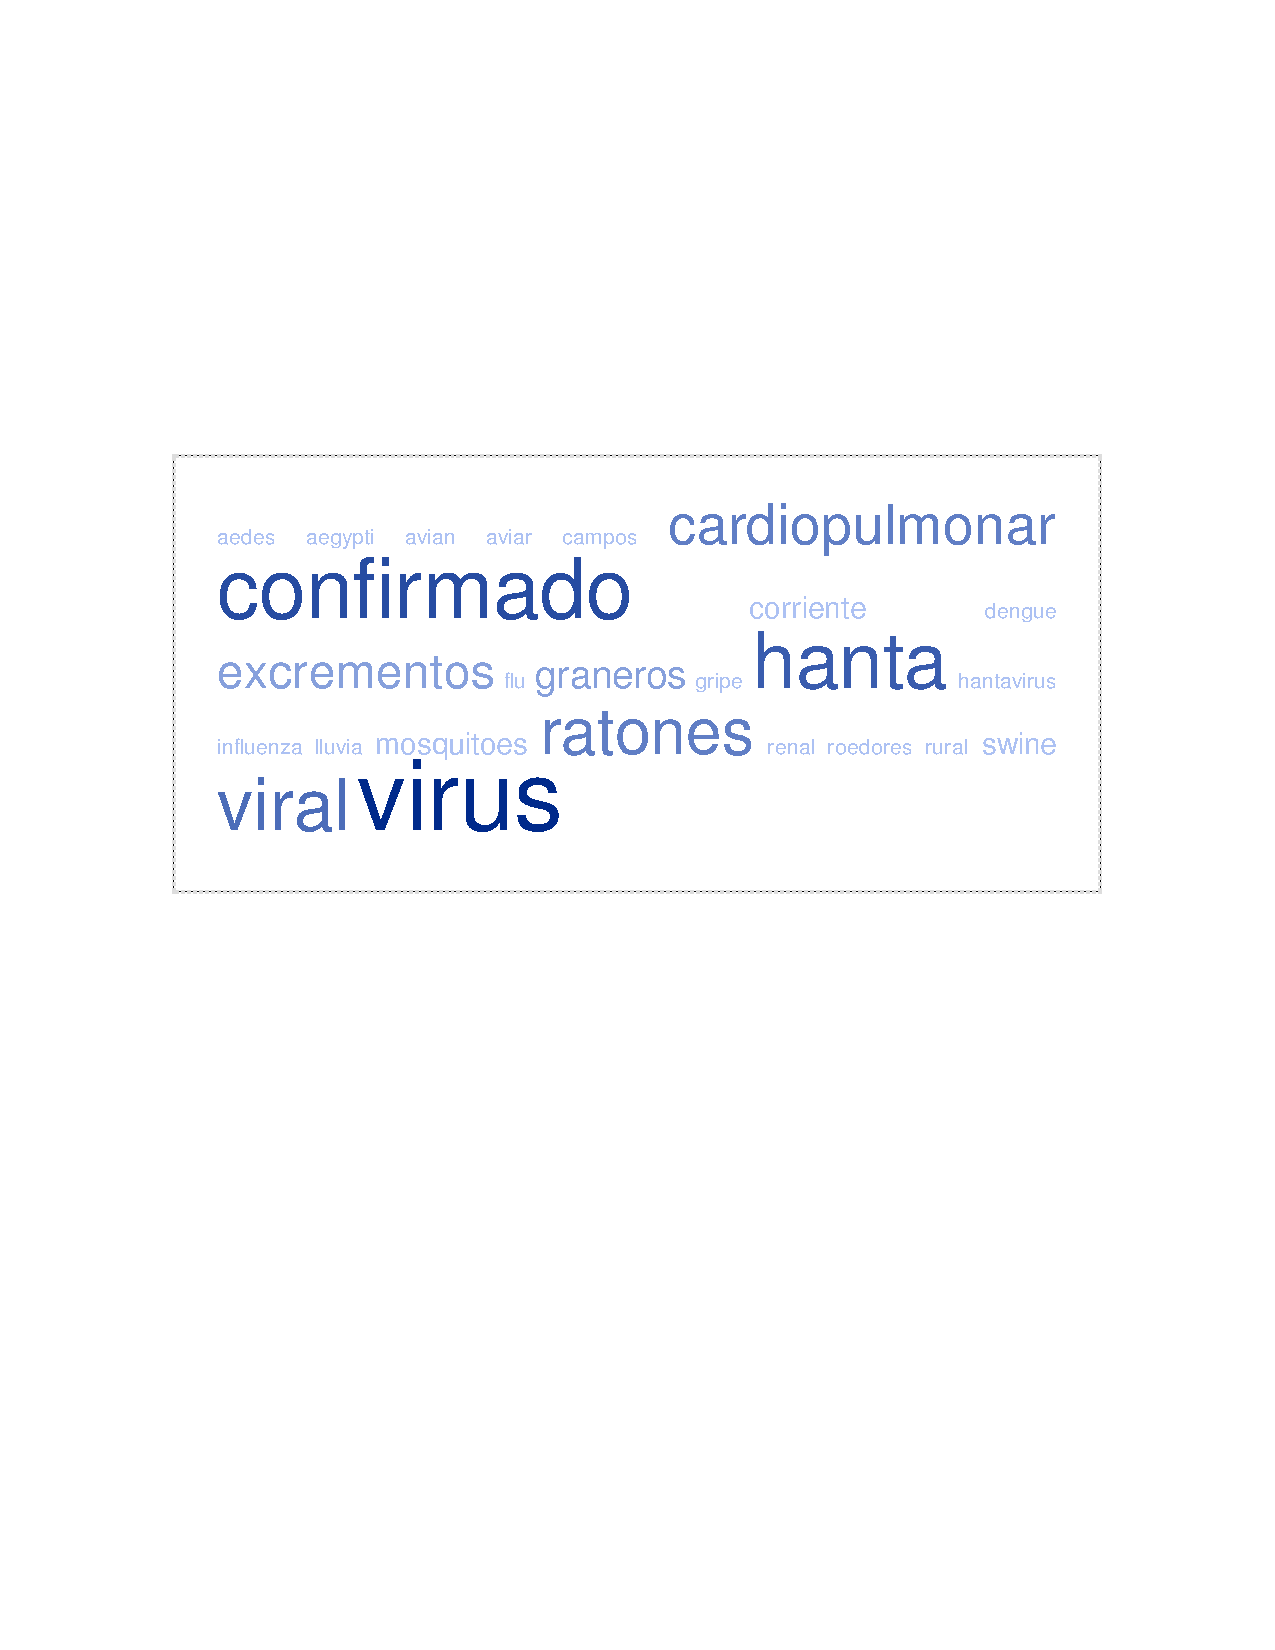
\includegraphics[scale=0.27]{figures/topic_2_cloud.pdf}\label{fig:topic_2_cloud}}
        \subfigure{
\includegraphics[scale=0.27]{figures/topic_7_cloud.pdf}\label{fig:topic_7_cloud}}
        \subfigure{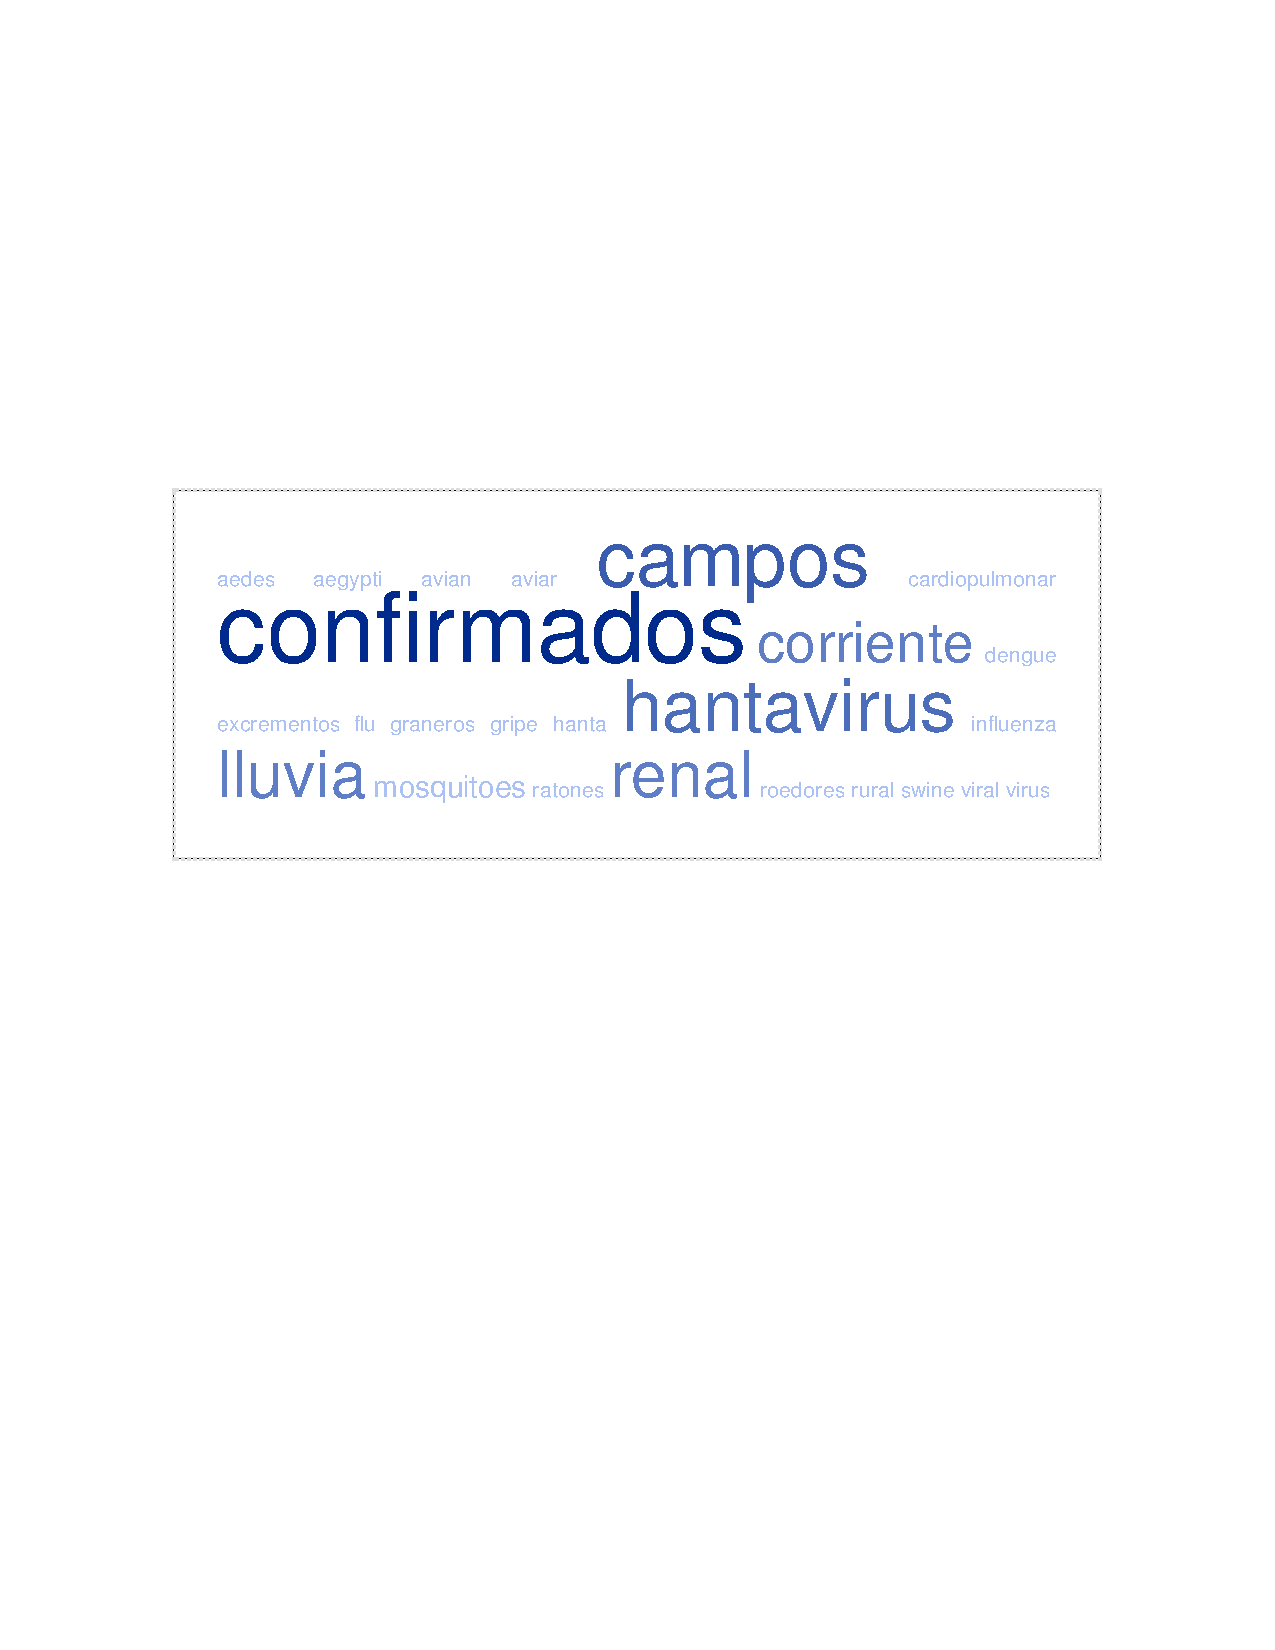
\includegraphics[scale=0.27]{figures/topic_11_cloud.pdf}\label{fig:topic_11_cloud}}
\end{center}
\caption{Word Clouds of Hantavirus Topics (a) Topic 2 (b) Topic 7 (c) Topic 11}
\label{fig:Rare_clouds}
\end{figure*}

\begin{figure*}[ht]
\begin{center}
        \subfigure{
\includegraphics[scale=0.27]{figures/topic_2_1.pdf}\label{fig:topic_2_1}}
        \subfigure{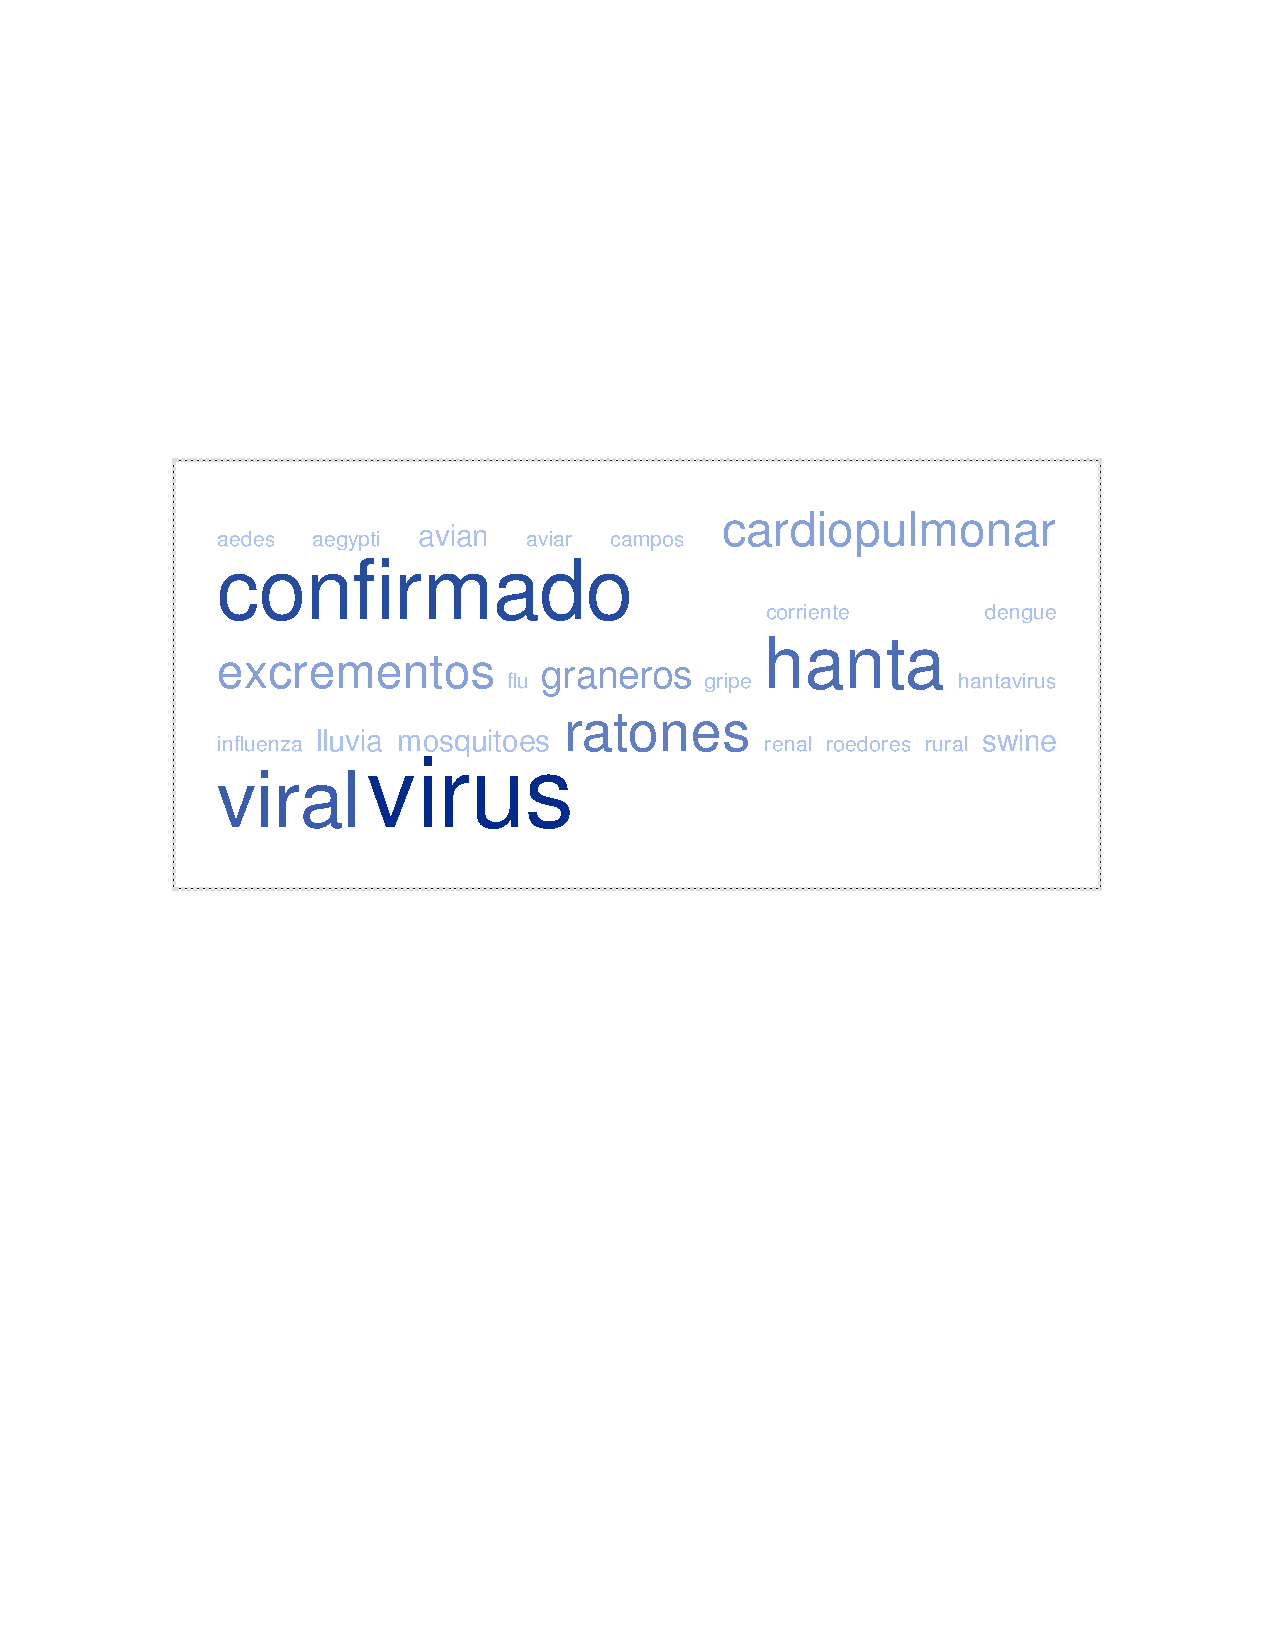
\includegraphics[scale=0.27]{figures/topic_2_2.pdf}\label{fig:topic_2_2}}
        \subfigure{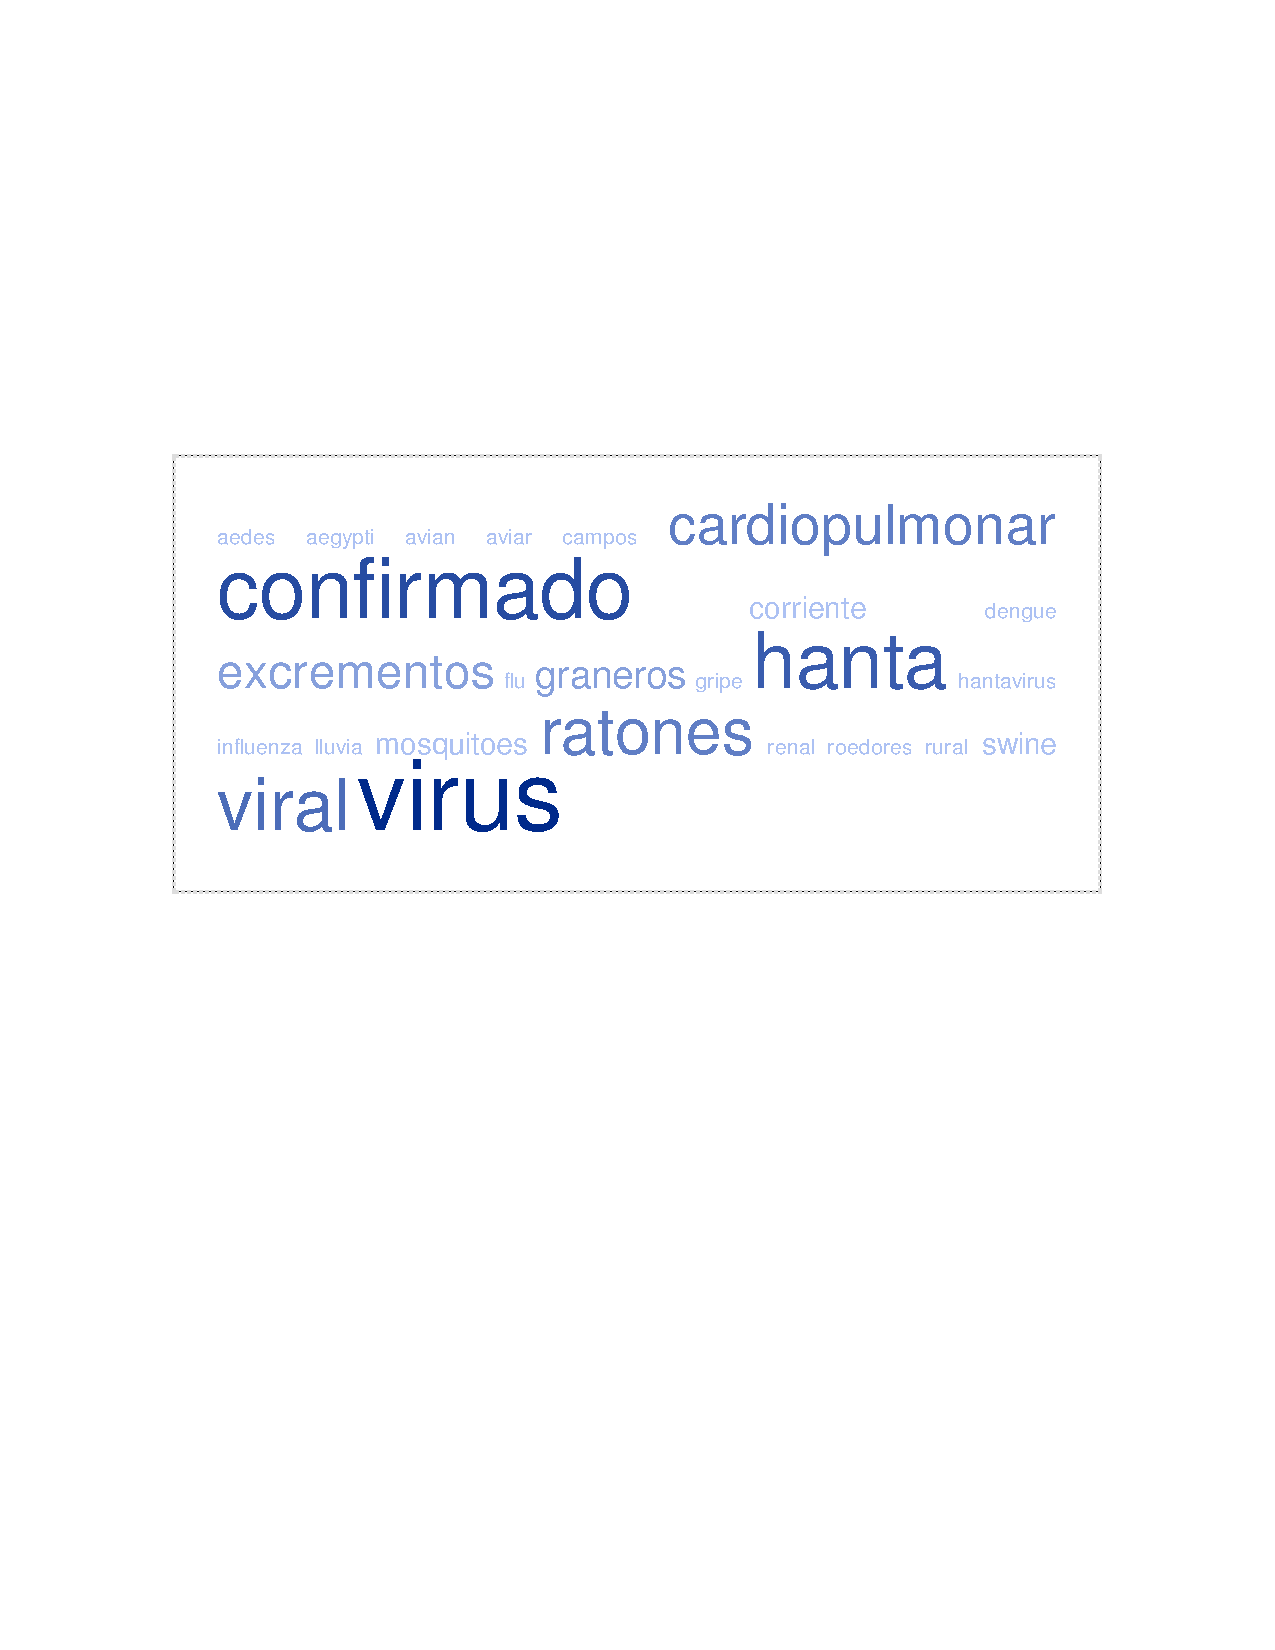
\includegraphics[scale=0.27]{figures/topic_2_cloud.pdf}\label{fig:topic_2_cloud}}
\end{center}
\caption{Evolution of Hantavirus Topic (Topic 2) across the timeline (a)October 2012, (b) June 2013, (c) March 2014}
\label{fig:evolution_clouds}
\end{figure*}


Figures 3 and 4 show the keyword clouds for the disease topics discovered from the Healthmap corpus.
From the word clouds it is clear that the articles in the HealthMap corpus focus
on both common disease topics like "Swine Flu", "Avian Influenza", "Dengue" and rare disease topics
like "Hantavirus". Most of the keywords in the word clouds are in Spanish since 
we are analyzing the Latin American News Media.   

Since the focus of our work is forecasting Rare Disease (Hantavirus) outbreaks, 
our topics of interest are Topic 2, Topic 7 and Topic 11. The top-ranked keywords 
under these topics relate to "hanta", "ratones" (rats), "cardiopulmonar", "roedores" (rodents), "rural", 
"hantavirus", "excrementos" (rodent droppings), "graneros" (barns),
"campos" (fields), "lluvia" (rainfall) and "corriente" (water current). These keywords make 
sense as Hantavirus is mainly a cardiopulmonar disease caused by infection of rodents and/or rats 
in mainly rural areas (barns and fields). The infection is spread through rodent droppings, urine and saliva.
The population of rodents is influenced by Rainfall and 
thus increase in rainfall or water current is an indirect indicator of Hantavirus outbreaks.
Figure 5 shows the evolution of Topic 2 across timepoints (Ocotber
2012, June 2013, March 2014). It clearly depicts the fact that the hantavirus topics are becoming increasingly 
prominent as we train the Topic Model continuously with new incoming articles along the timeline.


\subsection{Disease Outbreak Detection Results}

For Disease Outbreak Detection we focus on four countries - Argentina,
Chile, Uruguay and Brazil for which Cases of hantavirus outbreaks were reported
from January 2013 to December 2013. Table 2 gives an
extensive evaluation of both our models (L-STAT and S-STAT) in terms of
forecasting Hantavirus incidences. As shown, the S-STAT model can
forecast hantavirus incidences with an average Lead Time of 6.4 days,
whereas the average Lead Time for L-Stat Model is 6.09 days. Both the
models are performing similar in terms of Lead Time. This can be
attributed to the similar manner by which both the models generate
warnings. In terms of Quality Score (QS), the S-STAT model is overall slighly
better than the L-STAT Model. Quality Score of S-STAT model is better than L-STAT for 6
months while L-STAT is superior in 5 months. This depicts that both the
approaches are more or less similar in forecasting Location and Time
accurately for certain hantavirus incidences. Finally, in terms of
F1-score S-STAT model completely outperforms the L-STAT model. F1-score
weights Recall and Precision equally, and thus a good model will
maximize both precision and recall simultaneously. As a result S-STAT is
a far better and reliable model than L-STAT in terms of Sensitivity and
Specificity. The reason is that the L-STAT model overpredicts, i.e. it
issues higher number of warnings than S-STAT for a particular country and  
a particular month. Over-predicting sometimes gives
advantage to the L-STAT model in terms of Quality Score(QS) because
higher number of warnings ensures higher number of matchings between
warnings and events and the best possible matching is selected while
calculating QS. Thats the reason L-STAT model is better than S-STAT in
terms of QS for certain months.

\begin{table}
  %\centering
  \caption{Performance results for S-STAT and L-STAT in terms of
  detecting hantavirus incidences}
  \begin{tabular}{|c|c|c|c|c|c|c|}
    \hline
    {\bf Month} & \multicolumn{3}{c|}{{\bf S-STAT}} &
    \multicolumn{3}{c|}{{\bf L-STAT}} \\
    \cline{2-7} & QS & LT & F1-score & QS & LT & F1-score \\
    \hline 
    {\bf Jan-2013} & 2.84 & 5.00 & 0.67 & 2.88 &
                      5.80 & 0.30 \\ 
    \hline
     {\bf Feb-2013} & 3.24 & 7.0 & 0.36 & 2.92 &
                      10.0 & 0.15 \\ 
    \hline
    {\bf March-2013} & 2.81 & 11.5 & 0.36 & 3.00 &
          7.25 & 0.57 \\ 
    \hline
    {\bf April-2013} & 2.99 & 5.0 & 0.53 & 2.85 &
                      5.67 & 0.35 \\ 
    \hline
    {\bf May-2013} & 3.01 & 4.25 & 0.43 & 2.99 &
                      4.33 & 0.18 \\ 
    \hline
    {\bf June-2013} & 2.72 & 6.0 & 0.23 & 0.00 &
                      0.00 & 0.00 \\ 
    \hline
    {\bf July-2013} & 2.92 & 5.0 & 0.19 & 0.00 &
                      0.00 & 0.00 \\ 
    \hline
    {\bf Aug-2013} & 2.72 & 2.0 & 0.21 & 2.81 &
                      12.00 & 0.26 \\ 
    \hline
    {\bf Sept-2013} & 2.47 & 5.0 & 0.49 & 2.44 &
                      5.5 & 0.21 \\ 
    \hline
    {\bf Oct-2013} & 2.97 & 9.6 & 0.59 & 3.17 &
                      10.75 & 0.19 \\ 
    \hline
    {\bf Nov-2013} & 2.65 & 6.8 & 0.62 & 2.87 &
                      4.67 & 0.23 \\ 
    \hline
    {\bf Dec-2013} & 2.87 & 8.0 & 0.64 & 2.87 &
                      7.1 & 0.53 \\ 
    \hline

  \end{tabular}
  \label{tab:results}
\end{table}

{\bf (*Table to be expanded, per country evaluation to be added, base rate
model results to be added, LS values to be given as a separate
evaluation metric*)}

\subsection{Model evaluation in capturing base rate changes in Chile and
argentina}

To be added.

\subsection{Analysis of Sources and/or Experts}

to be added.

\begin{figure*}[ht]
\begin{center}
        \subfigure{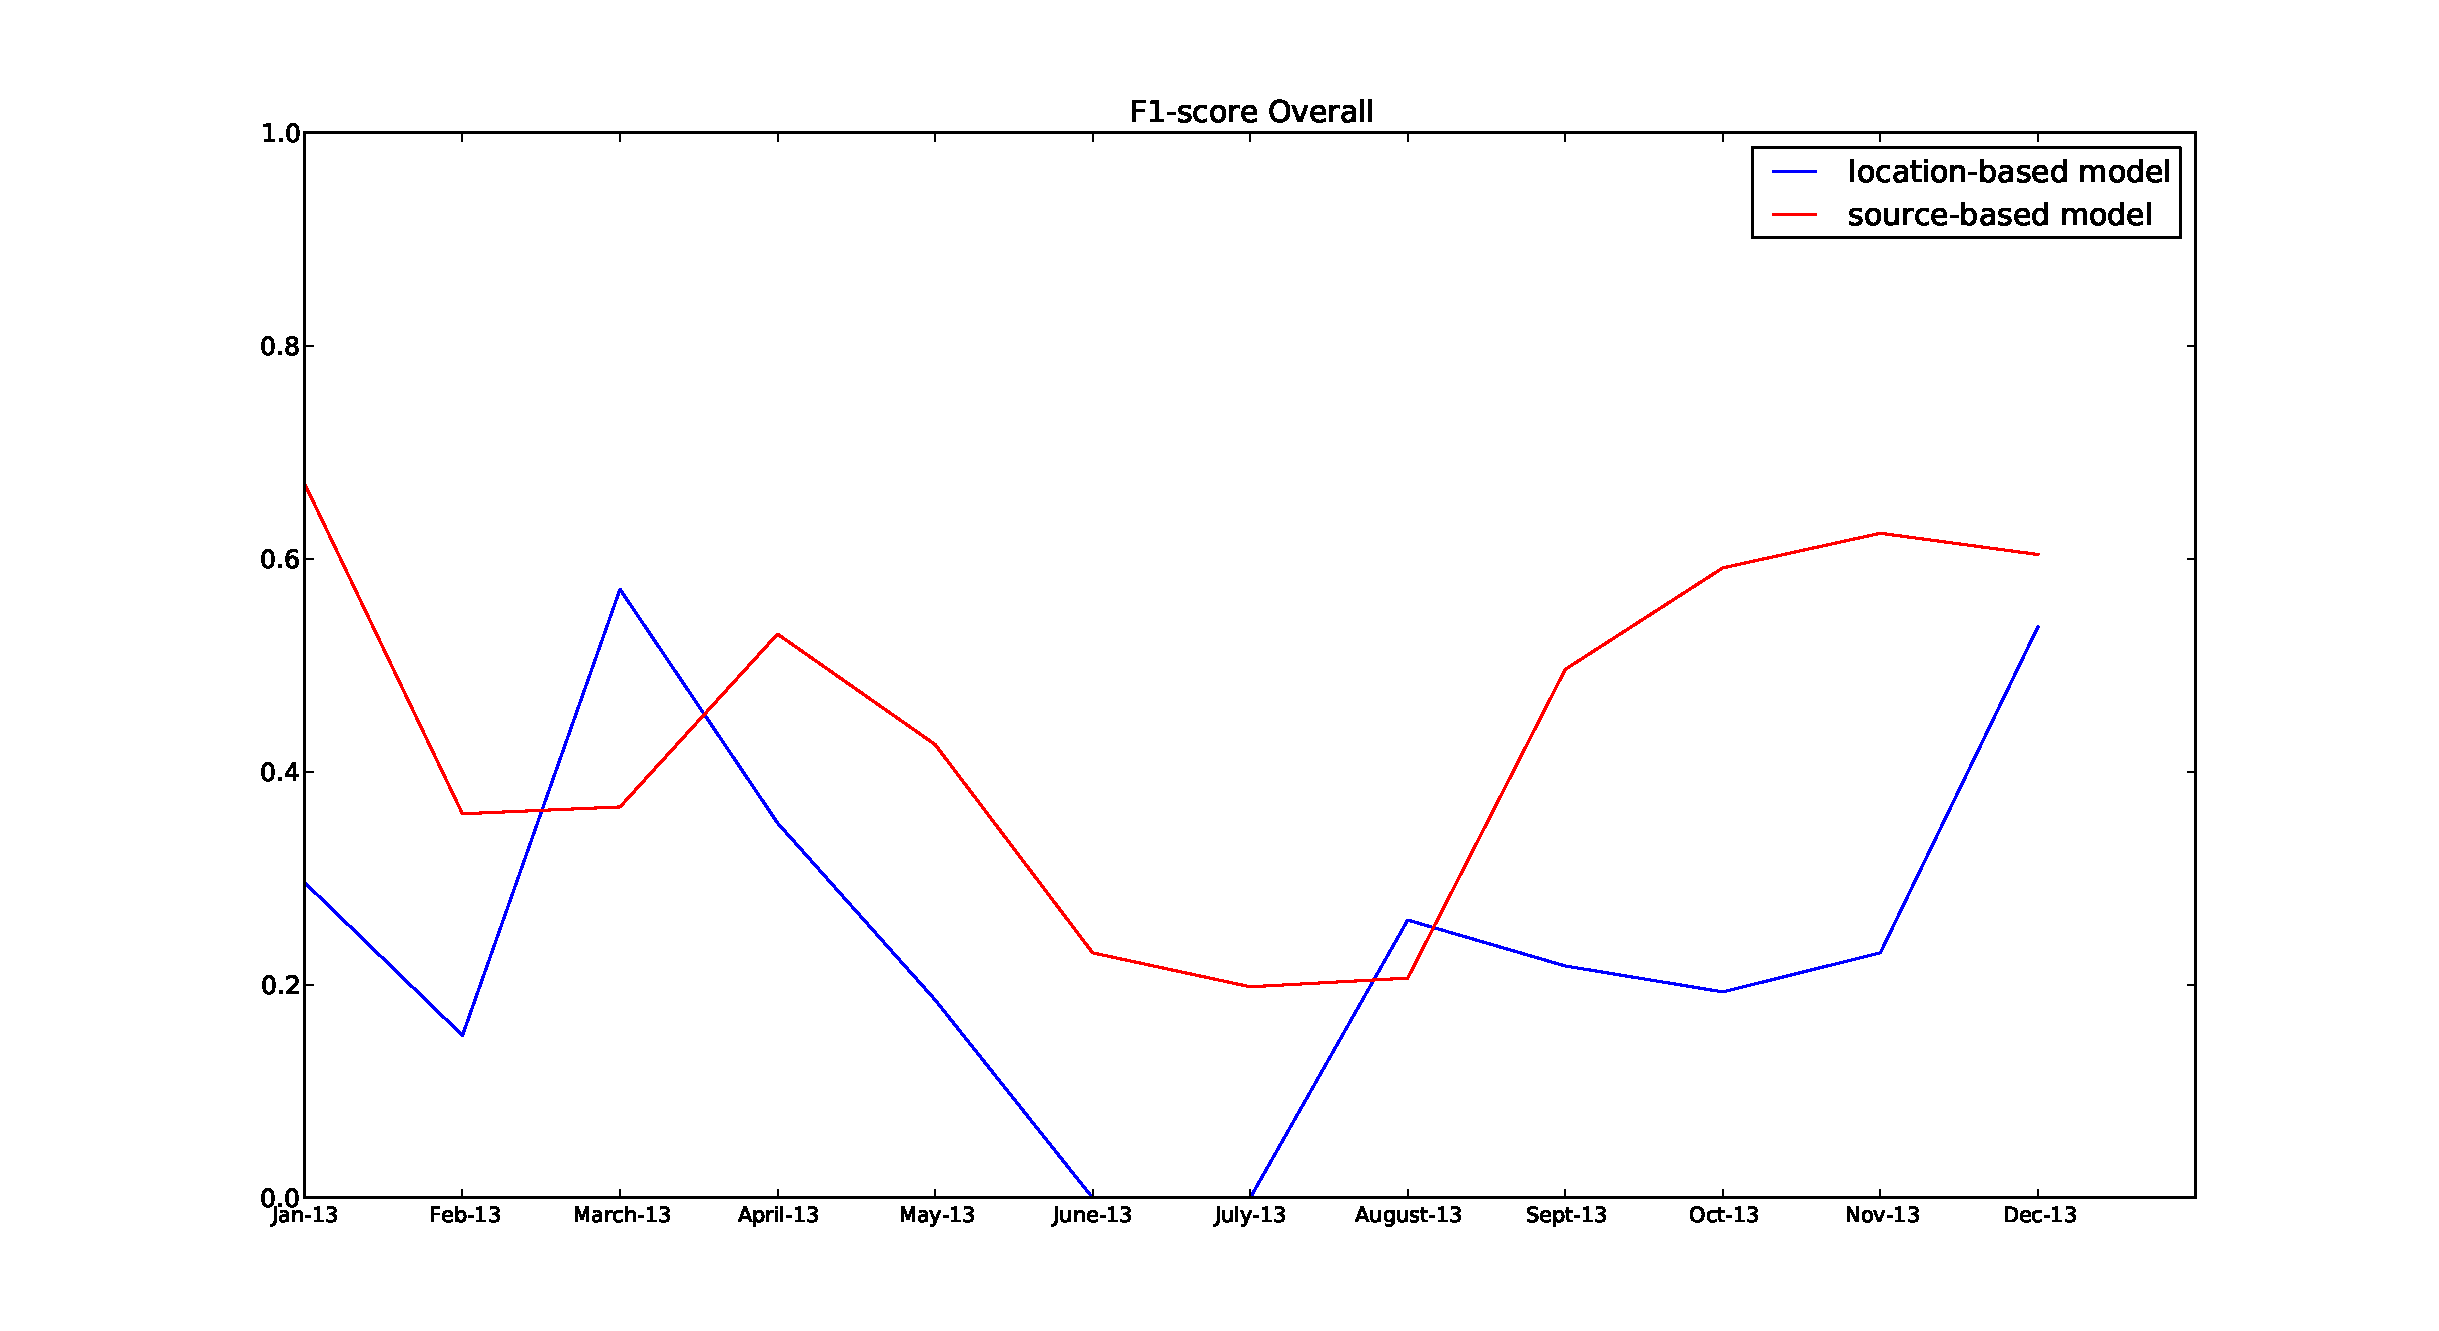
\includegraphics[scale=0.13]{figures/F1-score-overall.pdf}\label{fig:F1-score}}
        \subfigure{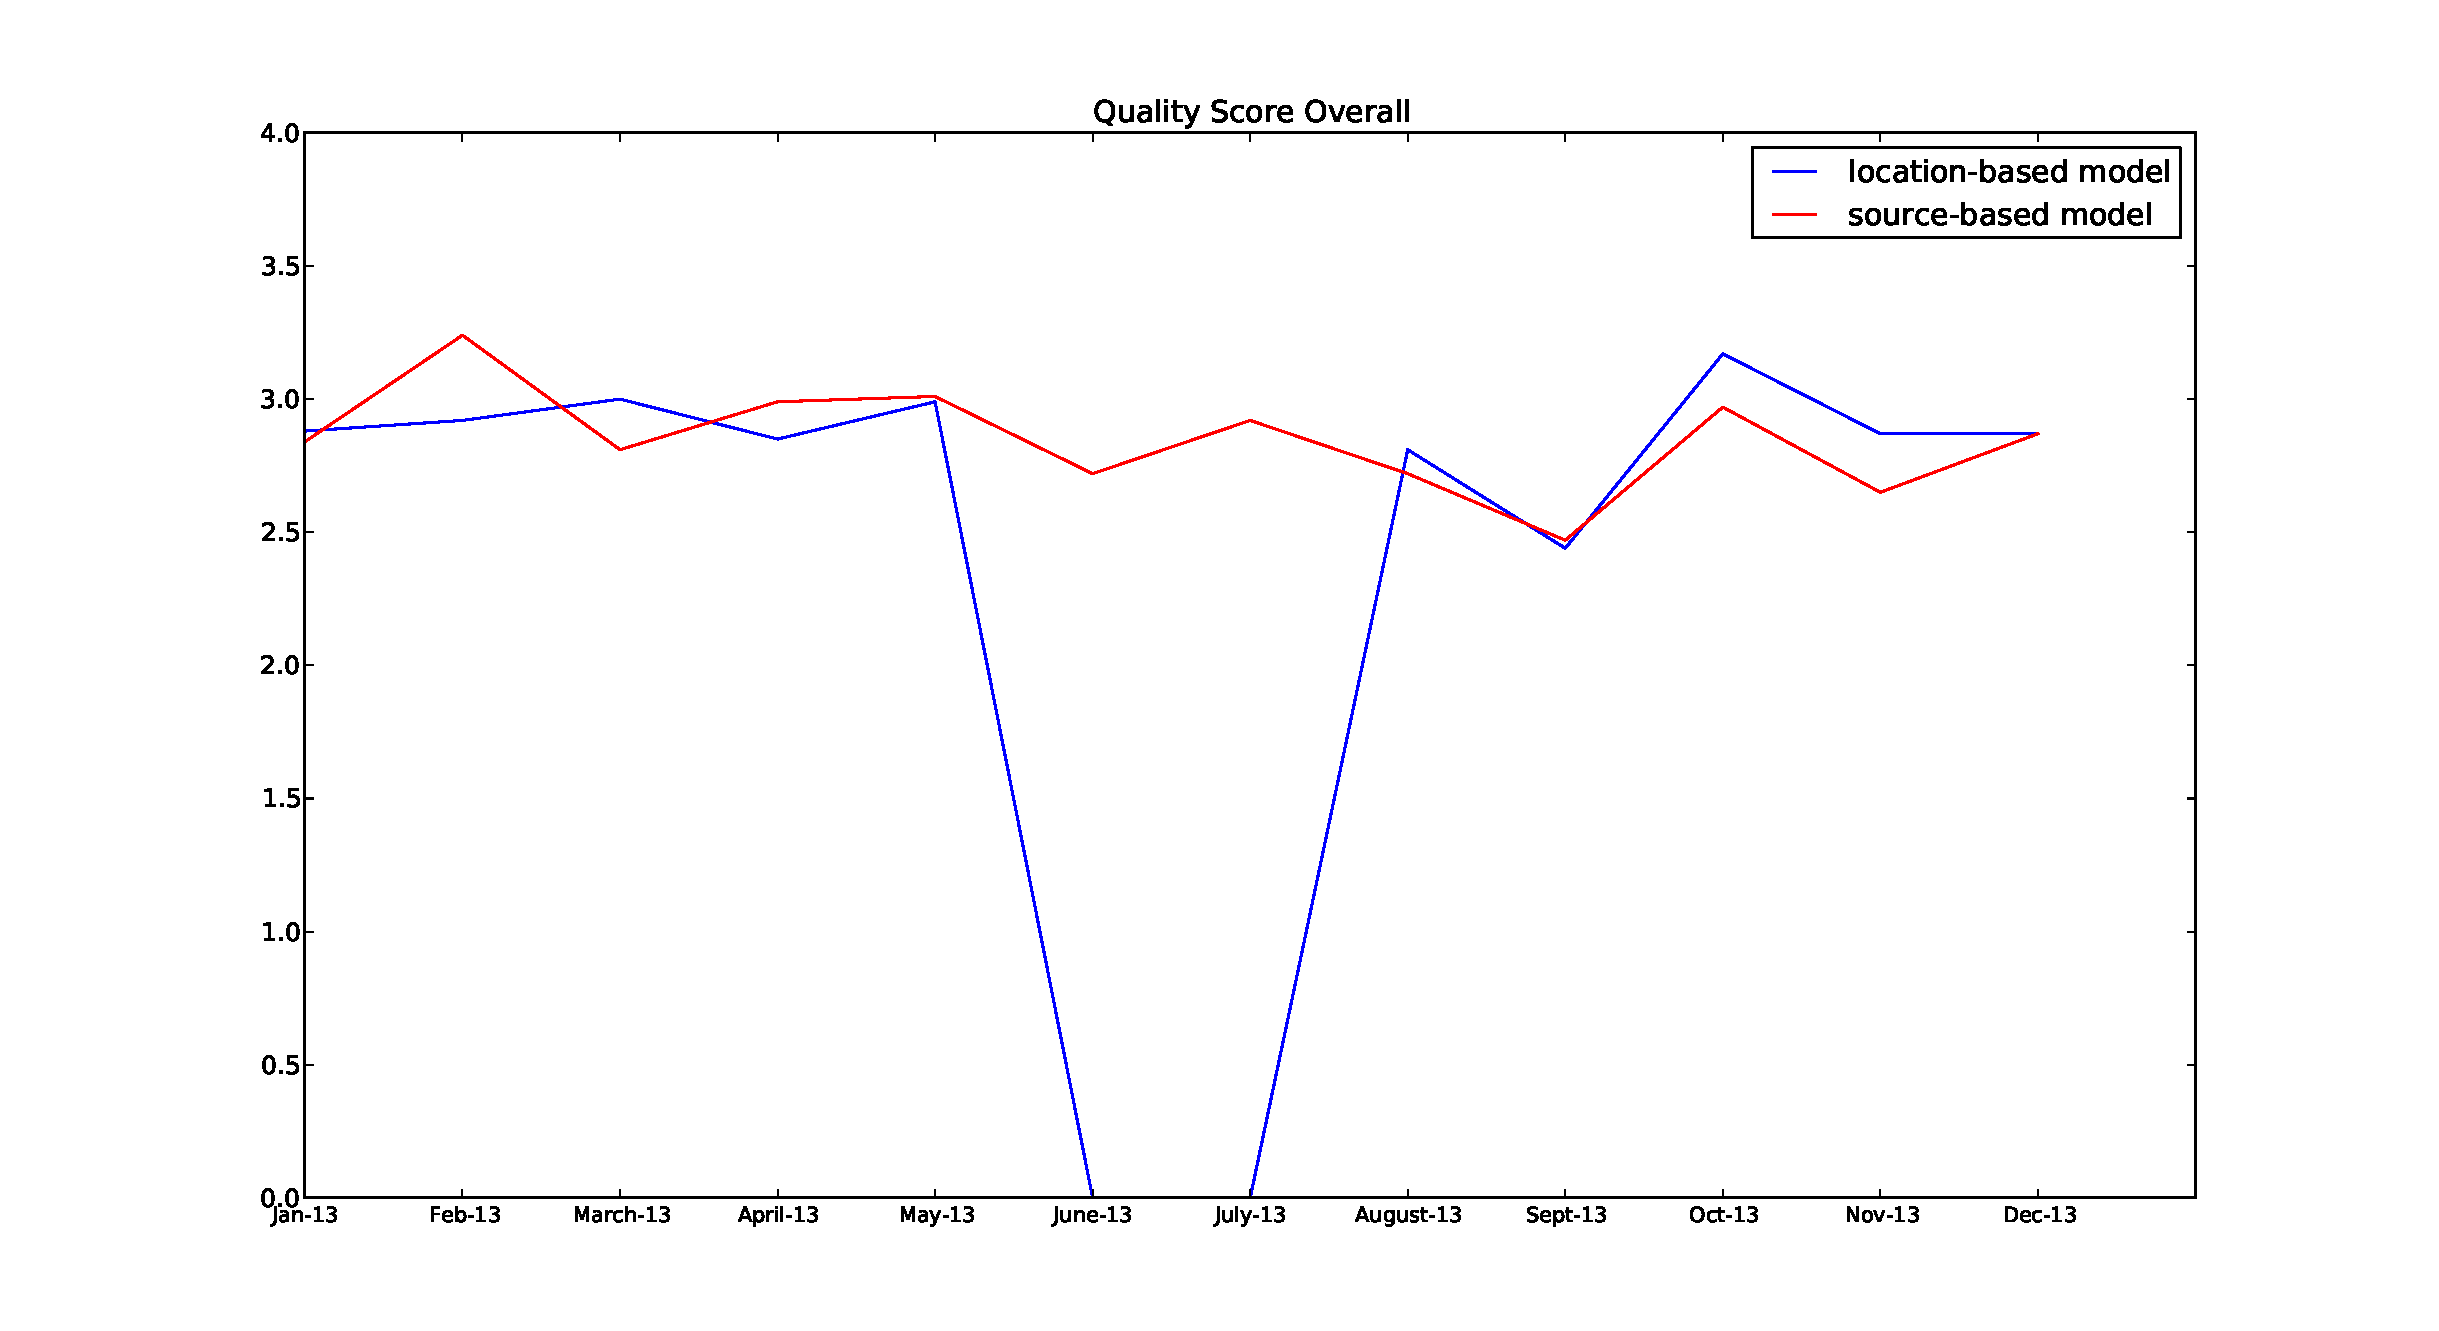
\includegraphics[scale=0.13]{figures/QS_overall.pdf}\label{fig:QS}}
        \subfigure{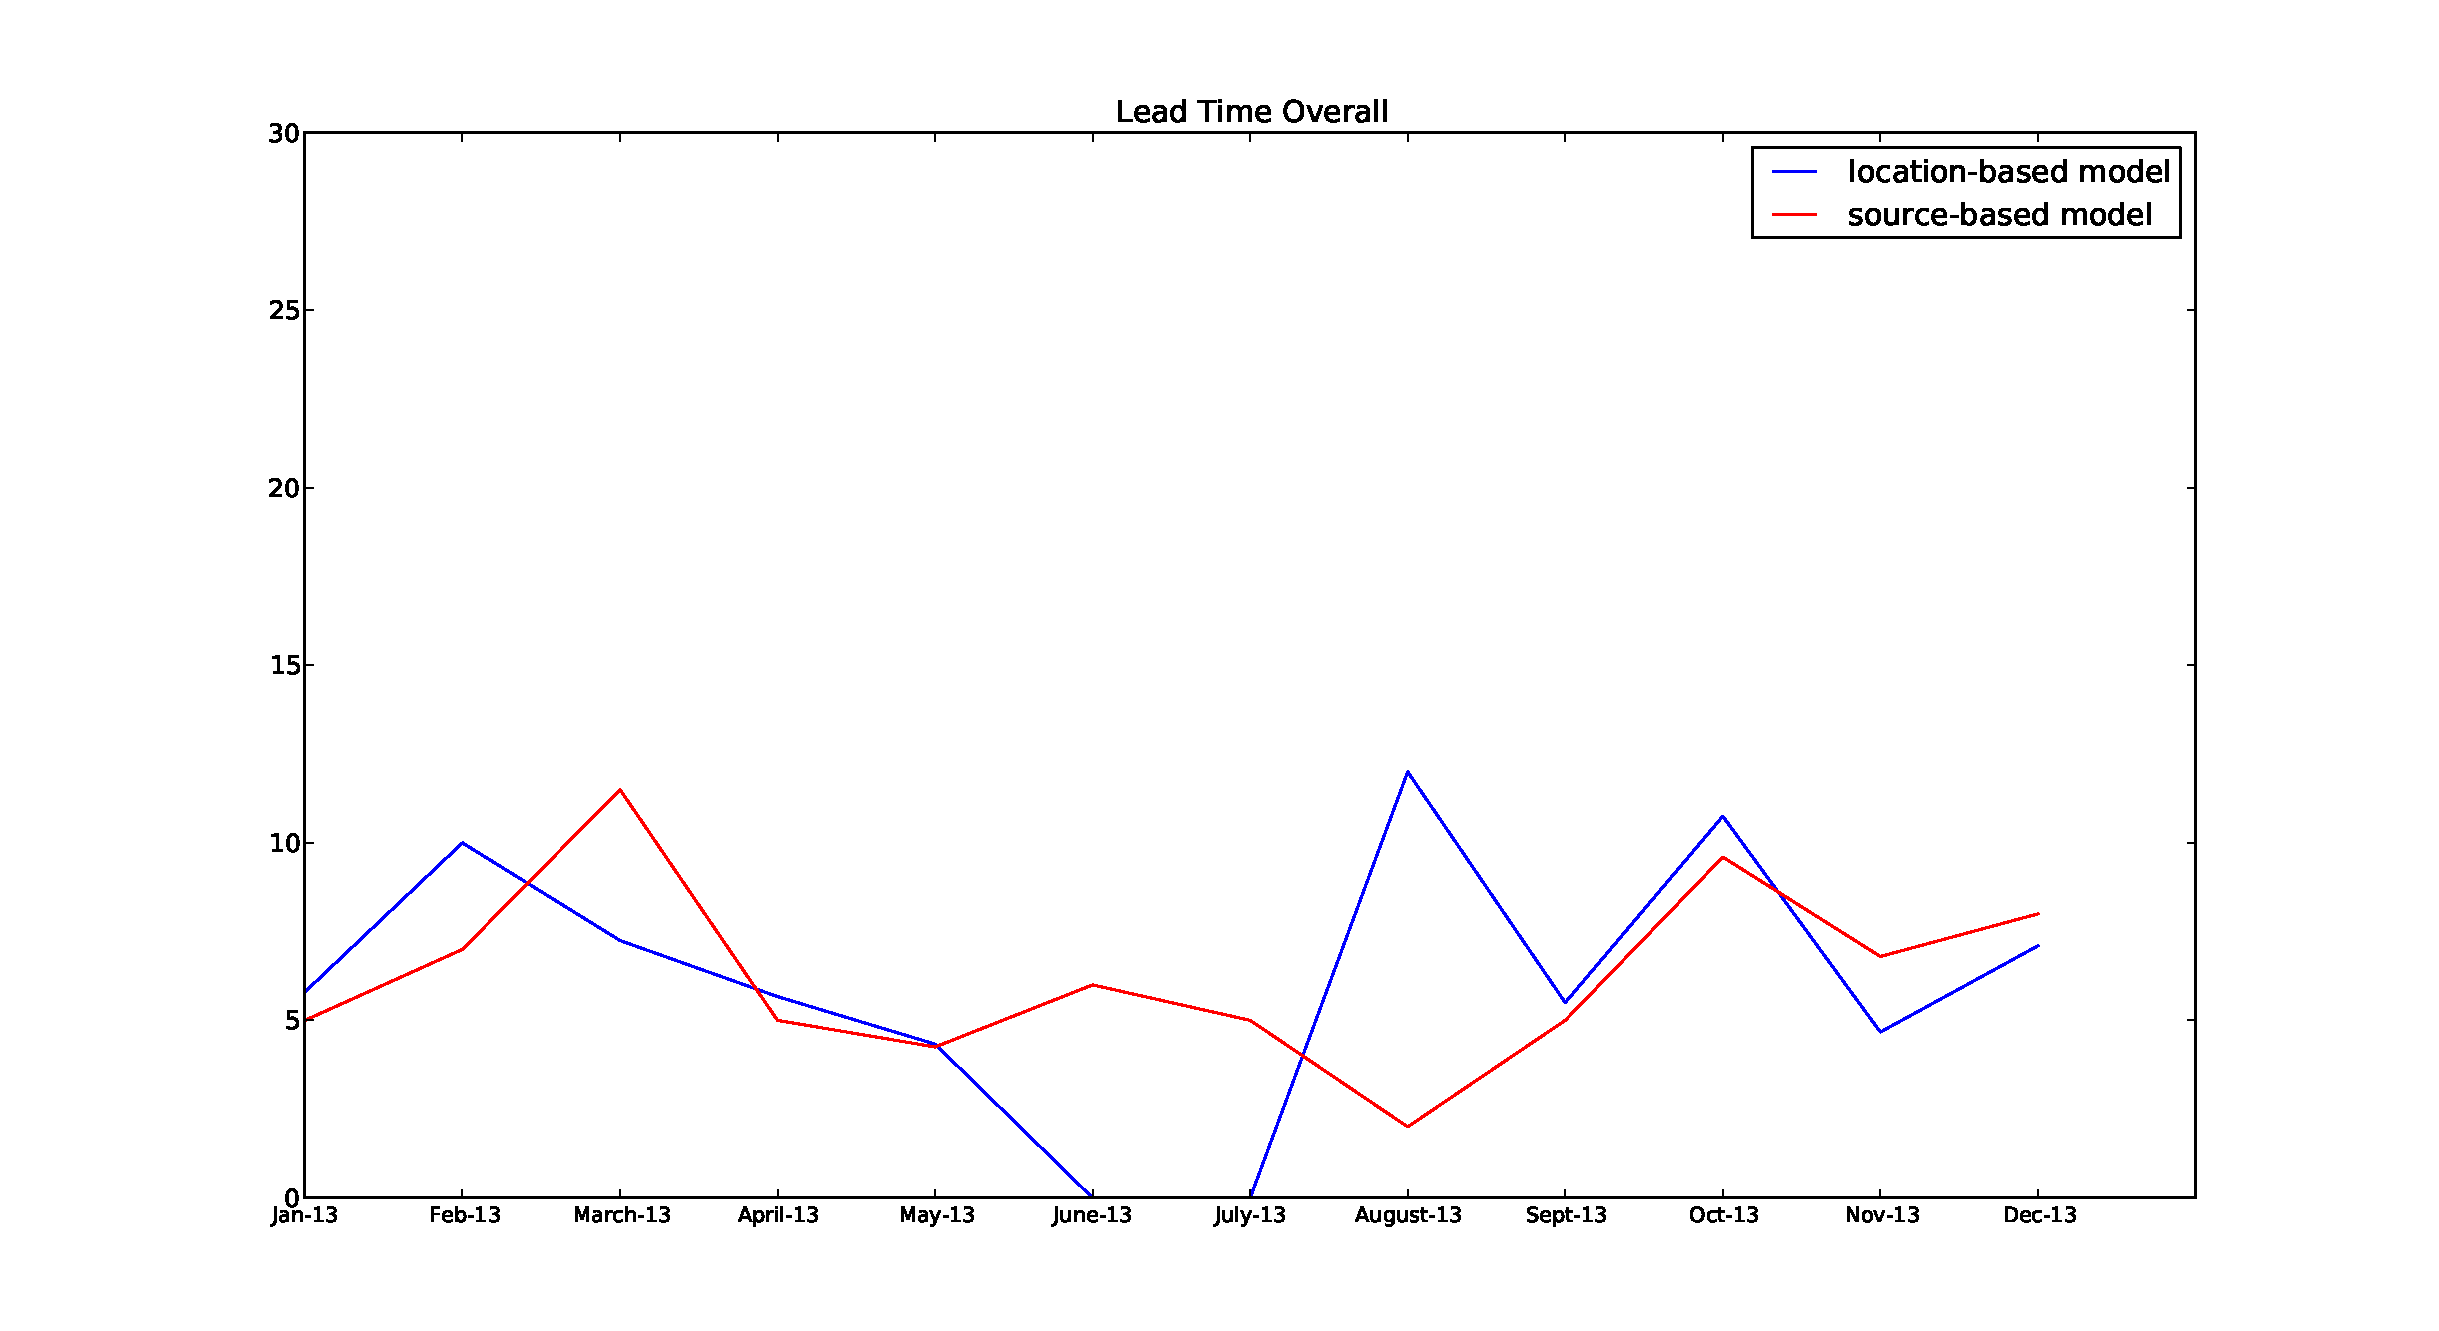
\includegraphics[scale=0.13]{figures/Lead_time_overall.pdf}\label{fig:LT}}
\end{center}
\caption{Comparison plots of S-STAT and L-STAT in terms of (a)
F1-score,(b) Quality Score and (c) Lead Time}
\label{fig:evaluation_metric}
\end{figure*}

\section{Related Work}
\label{sec:related_work}
Much of the work in the topic models literature has focused on identifying either spatial or temporal trends for the discovered topics. To the best of our knowledge most models focus on the temporal or spatial trends in isolation and do not analyze both types of trends jointly. 

A number of methods have been proposed for analyzing the time evolution of topics in document collections, such as the topics over time (TOT) model~\cite{wang:2006}, the dynamic topic model (DTM)~\cite{blei:2006}, and TriMine model~\cite{matsubara:2012}.  More precisely, TOT handles time-windows of fixed size and uses a Beta distribution to model the evolution of a topic over time. DTM  also focuses on a time-window of fixed size but uses Kalman filters to align topics with different time points. Finally, TriMine is able to analyze windows of variate size and unlike TOT and DTM is able to find cyclic time patterns with different timescales, which enables predicting future events. While TOT and DTM focus on the dimension of time alone, TriMine can associate the generation of different modalities with topics, however is agnostic to correlations across the different modalities.

A different line of work~cite{wang:2007} focuses on discovering spatial patterns jointly with the word co-occurrences. In particular, the authors introduced the Spatial Latent Dirichlet Allocation (SLDA), which better encodes spatial structure among words. While the model focuses on computer vision applications where documents are comprised by visual words the proposed techniques can be trivially extended to regular text documents. A similar approach was introduced by Ramage et al.~\cite{ramage:2009} for labeled documents where the labels can correspond to multiple modalities, i.e., locations as well.

Finally, although previous approaches~\cite{paul:11, sadilek:2012, rider:2013} have considered the use of topic models for detecting disease outbreaks, they mainly focus on common diseases, like influenza, for which large amounts of publicly available data or specialized medical records are available. 

\section{Conclusions}
\label{sec:conclusion}

\bibliographystyle{abbrv}
\bibliography{src_tm.bib}

\appendix
\section{Gibbs Sampling for \model}
\label{sec:gibbs}
In this section we first provide a Gibbs sampling algorithm for learning the parameters of the \model model. Before we proceed with the actual algorithm we present the joint distribution corresponding to the \model model. We have the following:
{\scriptsize
\begin{align}
&\Pr(\w,\tim,\loc,\z,{\bf \phi},{\bf \theta},{\bf \xi};\alpha,\beta,\gamma,\Psi) =  \nonumber \\
&=\prod_{z = 1}^{K}\Pr(\phi_z;\beta)\Pr(\xi_z;\gamma) \prod_{l = 1}^{L}\Pr(\theta_l;\alpha) \nonumber \\
& \cdot \prod_{s = 1}^{S}\prod_{i = 1}^{N_s} \Pr(z_{si}|l_{si},\theta_l)\Pr(l_{si}|\psi_s)\Pr(w_{si}|\phi_{z_{si}})\Pr(t_{si}|\xi_{z_{si}}) \nonumber
\end{align}}
Next, we marginalize over all ${\bf \phi}$, ${\bf \xi}$ and ${\bf \theta}$. We have:
{\scriptsize
\begin{align}
&\Pr(\w,\tim,\loc,\z;\alpha,\beta,\gamma,\Psi) =  \int_{\phi}\int_{\theta}\int_{\xi} \Pr(\w,\tim,\loc,\z,{\bf \phi},{\bf \theta},{\bf \xi};\alpha,\beta,\gamma,\Psi) d\xi d\theta d\phi \nonumber \\
&=\int_{\phi} \prod_{z = 1}^{K}\Pr(\phi_z;\beta) \prod_{s = 1}^{S}\prod_{i = 1}^{N_s}\Pr(w_{si}|\phi_{z_{si}}) d\phi \nonumber \\
& \cdot \int_{\xi} \prod_{z = 1}^{K} \Pr(\xi_z;\gamma)\prod_{s = 1}^{S}\prod_{i = 1}^{N_s}\Pr(t_{si}|\xi_{z_{si}}) d\xi \nonumber \\
&\cdot \int_{\theta} \prod_{l = 1}^{L}\Pr(\theta_l;\alpha)\prod_{s = 1}^{S}\prod_{i = 1}^{N_s}\Pr(z_{si}|l_{si},\theta_{l_{si}})\Pr(l_{si}|\psi_s) d\theta \nonumber \\
&=\int_{\phi} \prod_{z = 1}^{K}\Pr(\phi_z;\beta) \prod_{s = 1}^{S}\prod_{i = 1}^{N_s}\Pr(w_{si}|\phi_{z_{si}}) d\phi \nonumber \\
&  \cdot \int_{\xi} \prod_{z = 1}^{K} \Pr(\xi_z;\gamma)\prod_{s = 1}^{S}\prod_{i = 1}^{N_s}\Pr(t_{si}|\xi_{z_{si}}) d\xi \nonumber \\
&\cdot \int_{\theta} \prod_{l = 1}^{L}\Pr(\theta_l;\alpha)\prod_{s = 1}^{S}\prod_{i = 1}^{N_s}\Pr(z_{si}|l_{si},\theta_{l_{si}}) d\theta \prod_{s = 1}^{S}\prod_{i = 1}^{N_s} \Pr(l_{si}|\psi_s)\nonumber
\end{align}
}
We focus on the different integrals in the expression presented above. We start with the integral over ${\bf \phi}$. 
{\scriptsize
\begin{align}
& \int_{\phi} \prod_{z = 1}^{K}\Pr(\phi_z;\beta) \prod_{s = 1}^{S}\prod_{i = 1}^{N_s}\Pr(w_{si}|\phi_{z_{si}}) d\phi \nonumber \\
& =  \prod_{z = 1}^{K} \int_{\phi_{z}} \Pr(\phi_z;\beta) \prod_{s = 1}^{S}\prod_{i = 1}^{N_s}\Pr(w_{si}|\phi_{z_{si}}) d\phi_{z} \nonumber \\
&= \prod_{z = 1}^{K} \int_{\phi_z} \frac{\Gamma(\sum_{r = 1}^V \beta_r)}{\prod_{r = 1}^V \Gamma(\beta_r)}\prod_{r = 1}^V \phi_{zr}^{\beta_r -1} \prod_{r = 1}^V \phi_{zr}^{n^{z}_{(\cdot),r}} d\phi_z \nonumber \\
&= \prod_{z = 1}^{K} \int_{\phi_z} \frac{\Gamma(\sum_{r = 1}^V \beta_r)}{\prod_{r = 1}^V \Gamma(\beta_r)}\prod_{r = 1}^V \phi_{zr}^{\beta_r  + n^{z}_{r} -1} d\phi_z \nonumber \\
& = \prod_{z = 1}^K \frac{\Gamma(\sum_{r = 1}^V \beta_r)}{\prod_{r = 1}^V \Gamma(\beta_r)} \frac{\prod_{r = 1}^V \Gamma(n^{z}_{r} + \beta_r)}{\Gamma(\sum_{r =1}^V n^{z}_{r} + \beta_r)} \nonumber
\end{align}}
where $n^{z}_{r}$ denotes the number of times word $r$ was associated with topic $z$ across all sources and entries. Similarly we have for the $\xi$ part:
{\scriptsize
\begin{align}
&\int_{\xi} \prod_{z = 1}^{K} \Pr(\xi_z;\gamma)\prod_{s = 1}^{S}\prod_{i = 1}^{N_s}\Pr(t_{si}|\xi_{z_{si}}) d\xi \nonumber \\
&= \prod_{z = 1}^K \int_{\xi_z} \Pr(\xi_z;\gamma)\prod_{s = 1}^{S}\prod_{i = 1}^{N_s}\Pr(t_{si}|\xi_{z_{si}}) d\xi \nonumber \\
& = \prod_{z = 1}^K \frac{\Gamma(\sum_{t = 1}^T \gamma_t)}{\prod_{t = 1}^T \Gamma(\gamma_t)} \frac{\prod_{t = 1}^T \Gamma(m^{z}_{t} + \gamma_t)}{\Gamma(\sum_{t =1}^T m^{z}_{t} + \gamma_t)} \nonumber
\end{align}}
where $m^{z}_{t}$ denotes the number of times time-point $t$ was associated with topic $z$ across all sources. Finally, we focus on the $\theta$ integral. We follow a similar analysis and have the following:
{\scriptsize
\begin{align}
&\int_{\theta} \prod_{l = 1}^{L}\Pr(\theta_l;\alpha)\prod_{s = 1}^{S}\prod_{i = 1}^{N_s}\Pr(z_{si}|l_{si},\theta_{l_{si}}) d\theta \nonumber \\
&= \prod_{l = 1}^L \int_{\theta_l} \Pr(\theta_l;\alpha)\prod_{s = 1}^{S}\prod_{i = 1}^{N_s}\Pr(z_{si}|l_{si},\theta_{l_{si}}) d\theta_l \nonumber \\
& = \prod_{l =1}^L\int_{\theta_l} \frac{\Gamma(\sum_{z = 1}^K \alpha_z)}{\prod_{z = 1}^K \Gamma(\alpha_z)}\prod_{z = 1}^K \theta_{lz}^{\alpha_z -1}\prod_{z=1}^K\theta_{lz}^{o^z_{l}}d\theta_l \nonumber \\
&= \prod_{l =1}^L\int_{\theta_l} \frac{\Gamma(\sum_{z = 1}^K \alpha_z)}{\prod_{z = 1}^K \Gamma(\alpha_z)}\prod_{z = 1}^K \theta_{lz}^{\alpha_z  + o^z_{l}-1}d\theta_l \nonumber \\
& = \prod_{l =1}^L\frac{\Gamma(\sum_{z = 1}^K \alpha_z)}{\prod_{z = 1}^K \Gamma(\alpha_z)}\frac{\prod_{z=1}^K\Gamma(o^z_l + \alpha_z)}{\Gamma(\sum_{z = 1}^K o^z_l + \alpha_z)}\nonumber
\end{align}}
where $o^z_l$ denotes the number of times location $l$ was associated with topic $z$ across all sources and their entries. 
Eventually we have that the joint distribution is given by:
{\scriptsize
\begin{align}
&\Pr(\w,\tim,\loc,\z;\alpha,\beta,\gamma,\Psi) = \prod_{z = 1}^K \frac{\Gamma(\sum_{r = 1}^V \beta_r)}{\prod_{r = 1}^V \Gamma(\beta_r)} \frac{\prod_{r = 1}^V \Gamma(n^{z}_{r} + \beta_r)}{\Gamma(\sum_{r =1}^V n^{z}_{r} + \beta_r)} \nonumber \\
&\cdot \prod_{z = 1}^K \frac{\Gamma(\sum_{t = 1}^T \gamma_t)}{\prod_{t = 1}^T \Gamma(\gamma_t)} \frac{\prod_{t = 1}^T \Gamma(m^{z}_{t} + \gamma_t)}{\Gamma(\sum_{t =1}^T m^{z}_{t} + \gamma_t)} \nonumber \\
& \cdot \prod_{l =1}^L\frac{\Gamma(\sum_{z = 1}^K \alpha_z)}{\prod_{z = 1}^K \Gamma(\alpha_z)}\frac{\prod_{z=1}^K\Gamma(o^z_l + \alpha_z)}{\Gamma(\sum_{z = 1}^K o^z_l + \alpha_z)} \cdot \prod_{s = 1}^{S}\prod_{i = 1}^{N_s} \Pr(l_{si}|\psi_s) \nonumber
\end{align}}
The goal of Gibbs sampling is to approximate the conditional distribution $\Pr(\z | \w, \tim,\loc;\alpha,\beta,\gamma,\Psi)$. Using the chain rule we have the following for the conditional probability:
{\scriptsize
\begin{align}
&\Pr(z_{si}| \w,\tim,\loc,\z_{-si};\alpha,\beta,\gamma,\Psi) \nonumber \\
&= \frac{\Pr(z_{si}, w_{si}, t_{si}, l_{si}|\w_{-si},\tim_{-si},\loc_{-si},\z_{-si};\alpha,\beta,\gamma,\Psi)}{\Pr(w_{si}, t_{si}, l_{si}|\w_{-si},\tim_{-si},\loc_{-si},\z_{-si};\alpha,\beta,\gamma,\Psi)} \nonumber \\
& \propto \frac{n^{k,-(s,i)}_{w_{si}} + \beta_{w_{si}}}{\sum_{r = 1}^V n^{k,-(s,i)}_{r} + \beta_{r}} \cdot \frac{m^{k,-(s,i)}_{t_{si}} + \gamma_{t_{si}}}{\sum_{t = 1}^T m^{k,-(s,i)}_{t} + \gamma_{t}} \nonumber \\
& \cdot \frac{o^{k,-(s,i)}_{l_{si}} + \alpha_{l_{si}}}{\sum_{l = 1}^L o^{k,-(s,i)}_{l} + \alpha_{l}} \cdot \Pr(l_{si}|\psi_s) \nonumber
\end{align}}
where $-si$ in the superscript indicates that the current example has been excluded by the count summations. Notice that the probability $\Pr(l_{si}|\psi_s)$ is constant through all possible topic assignments and hence can be omitted. Eventually, we have that:
{\scriptsize
\begin{align}
&\Pr(z_{si}| \w,\tim,\loc,\z_{-si};\alpha,\beta,\gamma,\Psi) \nonumber \\
& \propto \frac{n^{k,-(s,i)}_{w_{si}} + \beta_{w_{si}}}{\sum_{r = 1}^V n^{k,-(s,i)}_{r} + \beta_{r}} \cdot \frac{m^{k,-(s,i)}_{t_{si}} + \gamma_{t_{si}}}{\sum_{t = 1}^T m^{k,-(s,i)}_{t} + \gamma_{t}} \nonumber \\
& \cdot \frac{o^{k,-(s,i)}_{l_{si}} + \alpha_{l_{si}}}{\sum_{l = 1}^L o^{k,-(s,i)}_{l} + \alpha_{l}}\nonumber
\end{align}}

\end{document}
